%; whizzy chapter
% -initex iniptex -latex platex -format platex -bibtex jbibtex -fmt fmt

%   Pdf作成手順
% dvipdfmx debianmeetingresume2005-fuyu.dvi
%  preview (shell-command "xpdf debianmeetingresume2005-fuyu.pdf&")

%この資料はA3用紙に一面あたり2頁両面印刷(一枚で4頁)で印刷する予定


%     Tokyo Debian Meeting resources
%     Copyright (C) 2006 Junichi Uekawa

%     This program is free software; you can redistribute it and/or modify
%     it under the terms of the GNU General Public License as published by
%     the Free Software Foundation; either version 2 of the License, or
%     (at your option) any later version.

%     This program is distributed in the hope that it will be useful,
%     but WITHOUT ANY WARRANTY; without even the implied warranty of
%     MERCHANTABILITY or FITNESS FOR A PARTICULAR PURPOSE.  See the
%     GNU General Public License for more details.

%     You should have received a copy of the GNU General Public License
%     along with this program; if not, write to the Free Software
%     Foundation, Inc., 51 Franklin St, Fifth Floor, Boston, MA  02110-1301 USA


\documentclass[mingoth,a4paper]{jsarticle}
\usepackage[dvipdfmx]{graphicx}
\usepackage{fancybox}
\usepackage{longtable}
\usepackage{ascmac}	% 囲み (screen,itembox)
\usepackage{fancyvrb}   % 囲み Verbatim のために必要
\usepackage[dvipdfmx]{hyperref}
\usepackage{url}

%http://www.naney.org/diki/dk/hyperref.html
%日本語EUC系環境の時
\AtBeginDvi{\special{pdf:tounicode EUC-UCS2}}
%シフトJIS系環境の時
%\AtBeginDvi{\special{pdf:tounicode 90ms-RKSJ-UCS2}}

%% spacing の設定をする。枠を減らす。
\setlength\headheight{0mm}
\setlength\topmargin{-20mm}
\setlength\headsep{0mm}
\setlength\topskip{3mm}
\setlength\maxdepth{4pt}
\setlength\columnsep{6mm}
\setlength\textheight{252mm}
\setlength\topmargin{-5mm}
\setlength\textwidth{170mm}
\setlength\oddsidemargin{-5mm}
\setlength\evensidemargin{-5mm}

% とりあえずcommandline環境を定義。入出力についてはcommandline環境を活用
%する
\newenvironment{commandline}%
{\VerbatimEnvironment
  \begin{Sbox}\begin{minipage}{15cm}\begin{fontsize}{7.3}{7.3} \begin{BVerbatim}}%
{\end{BVerbatim}\end{fontsize}\end{minipage}\end{Sbox}
  \setlength{\fboxsep}{8pt}\fbox{\TheSbox}}


%%% start of santaku
\makeatletter
\newwrite\tf@jqz
\immediate\openout\tf@jqz\jobname.jqz\relax
\makeatother
\newcounter{santakucounter}
\newcommand{\santaku}[5]{%
\addtocounter{santakucounter}{1}

\addtocontents{jqz}{\arabic{santakucounter}. #5\\}
\nopagebreak 問題\arabic{santakucounter}. 
#1\\
\nopagebreak□ A #2\\
\nopagebreak□ B #3\\
\nopagebreak□ C #4
\pagebreak[1]
\hspace{1cm}
\\

}
%%% end of santaku


\newcommand{\emptyspace}{(\underline{\hspace{1cm}})}



\newcommand{\subsubsubsection}[1]{%
\vspace{1zw}{\bf #1}\\}


% sectionをセンタリングする
\makeatletter
  \renewcommand{\section}{\@startsection{section}{1}{\z@}%
    {\Cvs \@plus.5\Cdp \@minus.2\Cdp}% 前アキ
    {.5\Cvs \@plus.3\Cdp}% 後アキ
    {\normalfont\Large\headfont\raggedright\centering}} % style
\makeatother

% section の代わりの環境
\newcommand{\dancersection}[2]{%
\newpage
東京エリアDebian勉強会 2005 夏
\hrule
\vspace{0.5mm}
\hrule
\hfill{}\includegraphics[width=3cm]{image200502/openlogo-nd.eps}\\
\vspace{-4cm}
\begin{center}
  \section{#1}
\end{center}
\hfill{}#2\hspace{3cm}\space\\
\hrule
\hrule
\vspace{1cm}
}

%% for gotom
\newenvironment{gdescription}%  
{%
   \begin{list}{}% 見出し記号/直後の空白を調節
   {%
      \setlength{\itemindent}{0mm}
      \setlength{\leftmargin}{45mm}%  左のインデント
      \setlength{\rightmargin}{0zw}% 右のインデント
      \setlength{\labelsep}{4mm}%    黒丸と説明文の間
      \setlength{\labelwidth}{4cm}%  ラベルの幅
      \setlength{\itemsep}{0em}%     項目ごとの改行幅
      \setlength{\parsep}{0cm}%      段落での改行幅
      \setlength{\listparindent}{0cm}% 段落での一字下り
      \let\makelabel\gdescriptionlabel
   }
}{%
   \end{list}%
}
\newcommand*\gdescriptionlabel[1]{\hspace\labelsep\normalfont\bfseries #1}
%%

\begin{document}

\begin{titlepage}
% 毎月変更する部分
\title{%\includegraphics[width=9cm]{image200502/openlogo-nd.eps}\\
あんどきゅめんてっどでびあん 2005年冬号}
\date{}
\author{\bf 東京エリアDebian勉強会} 
%\maketitle  % use the graphics instead of the text

\includegraphics[height=252mm]{image2005-fuyu/titlepage-winter.eps}
%\thispagestyle{empty}
\end{titlepage}

\newpage
\setcounter{tocdepth}{1}
\tableofcontents
\vspace{6cm}

\large
\begin{itembox}{\bf『あんどきゅめんてっど でびあん』について}
本書は、東京周辺で毎月行なわれている『東京エリア Debian 勉強会』で
使用された資料・小ネタ・必殺技などを一冊にまとめたものです。
収録範囲は勉強会第7回から第10回まで。
内容は無保証、つっこみなどがあれば勉強会にて。
\end{itembox}
\normalfont


\dancersection{ITPの仕方からアップロードまでの流れ}{岩松 信洋}
\label{sec:iwamatsu}
\subsection{はじめに}

    今回、「このソフトウェアをDebianパッケージにしてDebianの一部として提供したい」と
    思ってるんだけどどうしたらよいのか、
    Debian Developer ではない人の視点から、ITPをどのように行えばいいのかまとめてみました。
	
\subsection{ITPとは}

    Intend To Package の略で 新しく Debian にパッケージを提供したいときに BTS に登録します。
    これはDebian Developer でなくても 行うことができます。
	
\subsection{ITPをする前に}

    ITPをする前に チェックしておかなければいけないことがあります。
	
  	\begin{enumerate}
  	\item パッケージ化したいソフトウェアのライセンスをチェックします。
	
        Debian は Debian フリーソフトウェアガイドライン ( DFSG ) に準じているソフトウェアでない
        といけません。"GPL"、"BSD"、および "Artistic" がそのライセンスの例になります。

    \item もうすでにパッケージがある可能性があるのでチェックする。
	
        {\bf \url{http://www.debian.org/distrib/packages} } や {\bf apt-cache search }で確認することができます。
		
        パッケージ化されていても Orphaned ( みなしご化 ) されていることもあります。
		
        {\bf \url{http://www.debian.org/devel/wnpp/orphaned} }で確認することができます。

        ITA (Intent To Adopt ) をして引き取ってメンテナンスをしましょう。

    \item ITP されていないか確認する。
	
        もうすでに パッケージにしたいソフトウェアが ITP されている可能性があります。

        {\bf \url{http://www.debian.org/devel/wnpp/being_packaged} }で確認することができます。

    \item RFPされていることをチェックする。
	
        Request For Package の略でパッケージ化の要望がBTSされていることがあります。

        {\bf \url{http://www.debian.org/devel/wnpp/requested} }で確認することができます。
		
        RFP されているときは バグの内容を RFP から ITP に変更する必要があります。

    \item Debianパッケージにしてみる。
	
        提供したいソフトウェアをDebianパッケージにしましょう。
        ITPしてからパッケージ化してもいいと思いますが、先におこなっておいて不具合がないか調べておきましょう。
		
	\end{enumerate}
    これらをチェックして ITP をしましょう。

\subsection{ITPのしかた}
    実際にはどのようにITPをしたらよいのでしょうか。
    方法を以下にまとめてみました。

    \subsubsection{ ITP }
		\begin{enumerate}
        \item reportbug の起動
		\begin{verbatim}
% reportbug --email hoge@example.org wnpp
として reportbugを起動します。
--email でe-mail アドレスを指定します。
wnpp というのは Work-Needing and Prospective Packages の略です。
		\end{verbatim}
        \item バグリクエストタイプを聞かれるので ITP を選択します。
		\begin{verbatim}
1 ITP  This is an `Intent To Package'. Please submit a package description
       along with copyright and URL in such a report.
2 O    The package has been `Orphaned'. It needs a new maintainer as soon as
       possible.
3 RFA  This is a `Request for Adoption'. Due to lack of time, resources,
       interest or something similar, the current maintainer is asking for
       someone else to maintain this package. He/she will maintain it in the
       meantime, but perhaps not in the best possible way. In short: the
       package needs a new maintainer.
4 RFH  This is a `Request For Help'. The current maintainer wants to continue
       to maintain this package, but he/she needs some help to do this, because
       his/her time is limited or the package is quite big and needs several
       maintainers.
5 RFP  This is a `Request For Package'. You have found an interesting piece of
       software and would like someone else to maintain it for Debian. Please
       submit a package description along with copyright and URL in such a
       report.

Choose the request type: 1
\end{verbatim}

        \item パッケージ名を求められるので ITP したい パッケージ名を入力します。
		\begin{verbatim}
Please enter the proposed package name: hoge
		\end{verbatim}

        \item パッケージの簡単な説明を求められるので入力します。
		\begin{verbatim}

Checking status database...
Please briefly describe this package; this should be an appropriate short
description for the eventual package:
> hogehoge program
		\end{verbatim}

        \item 以下のような画面になるので、ソフトウェアの内容 ( バージョン、提供元Webサイト、ライセンス、説明文 ) を入力します。
		\begin{verbatim}
Subject: ITP: hoge -- hogehoge program
Package: wnpp
Owner: hoge <hoge@example.org>
Severity: wishlist


*** Please type your report below this line ***

* Package name    : hoge
  Version         : x.y.z
  Upstream Author : Name <somebody@example.org>
* URL             : http://www.example.org/
* License         : (GPL, LGPL, BSD, MIT/X, etc.)
  Description     : hogehoge program

  (Include the long description here.)

  -- System Information:
  Debian Release: testing/unstable
  APT prefers unstable
  APT policy: (500, 'unstable')
  Architecture: i386 (i686)
  Shell:  /bin/sh linked to /bin/bash
  Kernel: Linux 2.6.12
  Locale: LANG=ja_JP.eucJP, LC_CTYPE=ja_JP.eucJP (charmap=EUC-JP)
		\end{verbatim}

        \item 入力が終わると送信確認が行われます。
		\begin{verbatim}
Your report will be carbon-copied to debian-devel, per Debian policy.

Spawning sensible-editor...
No changes were made in the editor.
Report will be sent to "Debian Bug Tracking System" <submit@bugs.debian.org>
Submit this report on wnpp (e to edit) [y|n|a|c|E|i|l|m|p|q|?]?

			\end{verbatim}
            "y" を押すことによってサーバーに送信されます。
            これでITPの作業は終わりです。
		\end{enumerate}
    \subsubsection{ RFP → ITP }
        パッケージ化を希望されているパッケージをパッケージ化し、Debianに提供する方法です。
        RFPのバグに対してBTSします。
        実際にはタイトルをRFPからITPに変更します。

		以下のようなメールをバグ番号に対して送信します。
		バグコントロールメールサーバにコマンドを送信しています。
		
		\begin{verbatim}
        owner 283119 !	//! address を #bugnumber の「所有者」に設定
        retitle 283119 ITP: libflash -- GPL Flash (SWF) Library //! タイトルを変更する
        thanks //! コントロールサーバーへのコマンド終了

        Hi,

        I am interested in this package.
        I wish to adopt this package.

        Thanks,
         Iwamatsu
		\end{verbatim}
    \subsubsection{ O  →  ITA }
        みなしご化されているパッケージを引き取ってメンテナンスしたいときの方法です。
        Orphaned のバグに対してメールをします。
        実際にはタイトルをOからITAに変更します。
		
		以下のようなメールをバグ番号に対して送信します。
		バグコントロールメールサーバにコマンドを送信しています。

		\begin{verbatim}
        owner 283119 !	//! address を #bugnumber の「所有者」に設定
        retitle 283119 ITA: libflash -- GPL Flash (SWF) Library //! タイトルを変更する
        thanks	//! コントロールサーバーへのコマンド終了

        Hi,

        I am interested in this package.
        I wish to adopt this package.

        Thanks,
        Iwamatsu
		\end{verbatim}

		
\subsection{ITPしたら}

	\begin{enumerate}
    \item スポンサーを探す
        ITPをしたら スポンサーを探す必要があります。
        スポンサーとは スポンサーは現存する Debian Developer で 自分の指導者をしてくれる方です。
        Debian Developer でないとパッケージを Debian にアップロードすることができません。
        スポンサーは作成したパッケージをチェックし、パッケージをアップロードしてくれます。
        また、間違いがあるときは指摘をしてくれたり、アドバイスをしてくれます。
		
        スポンサーを探すには{\bf debian-mentors ML} で聞いてみるとよいでしょう。
		
        {\bf \url{http://lists.debian.org/debian-mentors/}}

        また、GPGキーサインでサインして頂いたDebian Developerの方に相談するのも方法のひとつです。
		
		
    \item スポンサーが見つかったら
        スポンサーが見つかったらそのスポンサーとやり取りし、パッケージを改善します。
		
        スポンサーがアップロードしてもいいと判断された場合、スポンサーの手によってDebian にアッ
        プロードされます。
	\end{enumerate}

\dancersection{debconf論}{鵜飼文敏\footnote{Fumitoshi UKAI, ukai@debian.or.jp, ukai@debian.org, Debian Project}}
\label{sec:ukai}
%%鵜飼さんの記事はここから
\subsection{はじめに}

debconfとは、Debianにおいてパッケージの設定を行なうためのフレームワー
クおよびそれを実装したパッケージです。そもそもは、元Debian Project
LeaderのWichert Akkerman発案のconfiguration database framework 構想
\footnote{/usr/share/doc/debian-policy/debconf\_specification.html}であり、
debconfは、それに基づくJoey Hessによる実装です。

従来、パッケージの設定のうち、パッケージメンテナがデフォルトを決めにくいもの、
つまりシステム管理者によって決定されるようなものは、メンテナスクリプト
\footnote{postinstなど}で、プロンプトをだし管理者が入力した値に基づい
て設定ファイルを生成するようにしていました。これはこれで非常に柔軟性が高い
\footnote{メンテナががんばってメンテナスクリプトを書けばいろいろできる} 
のですが、パッケージによって\footnote{メンテナによってというべきか?} 
やりかたが異なってしまい、ディストリビューションとしての統一感に欠けて
しまうという欠点がありました。また、パッケージのインストール時・アップ
グレード時に常に管理者の介在が必要になってしまうために、インストール・
アップグレード中にコンソールを離れているわけにはいかないという問題もは
らんでいます。

そこで考案されたのがdebconfです。debconfを使うことで設定データを統一して
扱うことができるようになります。

\subsection{debconfを使っているパッケージの設定の仕方}

apt-utilsをインストールしておくとapt-extracttemplatesを使って、パッケー
ジをダウンロードしてインストール作業をする前\footnote{unpackをする前}
にdebconfを使ってパッケージの設定をおこなうことができるようになります。
この時はdebconf自体の設定 debconf/frontend に従ったフロントエンド
\footnote{dialog,readlline,gnome,kde,editor,noninteractiveのどれか}をつかって
ユーザとのやりとりがおこなわれます。また、設定には優先度(priority)
\footnote{重要(critical)、高(high)、中(medium)、低(low)のどれか}が
つけられており、debconf/priority の値より優先度が高いものだけが
フロントエンドを介してユーザとやりとりをおこなわれるようになります。

またインストールした後もdpkg-reconfigureでパッケージの設定をしなおすこ
とができます。dpkg-reconfigureは、debconf/priorityの値にかかわらず低優
先度(low)\footnote{-pオプションを使わなければ}以上すなわちすべての設定
をやりなおすようになっています。

また、現在そのパッケージの設定値がどうなっているかを知りたい場合は
debconf-show コマンドが使えます。

\begin{commandline}
 # debconf-show debconf
 * debconf/priority: critical
 * debconf/frontend: Dialog
\end{commandline}


\subsection{debconfの裏側}

apt-getがパッケージをダウンロードしてくると/etc/apt/apt.conf.d/70debconfというファイルによりdpkg-preconfigure -aptが実行されるようになります。

\begin{commandline}
// Pre-configure all packages with debconf before they are installed.
// If you don't like it, comment it out.
DPkg::Pre-Install-Pkgs {"/usr/sbin/dpkg-preconfigure --apt || true";};
\end{commandline}

dpkg-preconfigureでは、apt-utilsのapt-extracttempaltesを使っているため、apt-utilsがインストールされていないと、debconfの設定はこのタイミングではおこなわれません。

dpkg-preconfigure -aptに対して、いまダウンロードしたパッケージのリストがわたされるので、それらからtemplateをとりだして configスクリプトの実行をおこないます。

\begin{itemize}
\item apt-getによる*.debのダウンロード。/var/cache/apt/archives/にパッケージがおかれる
\item dpkg-preconfigure -aptの実行
 \begin{itemize}
   \item /var/cache/apt/archives/からインストールしようとするdebをみつける
   \item control情報のtempaltesとconfigをとりだす\footnote{dpkg -I パッケージ.deb templates config。apt-extractpackageを使う}
   \item templatesをloadして、debconfデータベース\footnote{/var/cache/debconf/*.data}を更新
   \item configスクリプトを実行する。db\_set、db\_inputやdb\_go
 \end{itemize}
\item dpkg --unpack
 \begin{itemize}
 \item preinstを実行
 \item パッケージを展開し、ファイルをおきかえ
 \end{itemize}
\item dpkg --configure
 \begin{itemize}
 \item postinstを実行。db\_get
 \end{itemize}
\end{itemize}

基本的には、configスクリプトで設定情報を決定し\footnote{ユーザに対して設定情報をたずねるか、デフォルト値を設定する}、postinstスクリプトでそれを読みだして実際のパッケージの設定ファイルなどに書きだすという処理をおこなうことになります。

なお、debconfデータベースはregistryとして使うな\footnote{使うとdebconf abuseとしてbugをくらう}ので、debconfデータベースを参照するのはメンテナスクリプトだけにしておく必要があります。また、debconf以外で設定ファイルを変更された場合も、その情報を上書きすることなく反映する必要があります。

\begin{table}[htbp]
 \begin{tabular}[htbp]{|l|l|l|l|}\hline
 シェルコマンド & 内容 & データのむき & 使う場所 \\ \hline
 db\_version "2.0"& バージョンネゴシエーション & & \\ \hline
 db\_capb multiselect & キャパビリティネゴシエーション & & \\ \hline
 db\_title タイトル & タイトル文字列の設定 & スクリプト→ユーザ & config \\ \hline
 db\_stop & debconfの停止 & & postinst, postrm \\ \hline
 db\_input プライオリティ 変数名 & 変数への入力 & テンプレ→ユーザ→DB & config \\ \hline
 db\_go & 入力の実行 & & config \\ \hline
 db\_get 変数名 & 変数のとりだし & DB→スクリプト & postinst \\ \hline
 db\_set 変数名 値 & 変数の設定 & スクリプト→DB & config \\ \hline
 db\_reset 変数名 & 変数の初期化 & テンプレ→DB & \\ \hline
 db\_subst 変数名 鍵 置換 & 置き換え & テンプレ(←スクリプト) & config \\ \hline
 db\_fget 変数名 フラグ & フラグのとりだし & DB→スクリプト & \\ \hline
 db\_fset 変数名 フラグ 値 & フラグの設定 & スクリプト→DB & \\ \hline
 db\_metaget 変数名 フィールド & フィールドのとりだし & テンプレ→スクリプト & \\ \hline
 db\_register テンプレート 変数名 & 変数の生成 & 元テンプレ→テンプレ & config \\ \hline
 db\_unregister 変数名 & 変数の削除 & →テンプレ & \\ \hline
 db\_purge & データベースから削除 & →テンプレ、DB & postrm \\ \hline
 \end{tabular}
 \caption{debconfコマンド}
 \label{debconf:cmd}
\end{table}

debconfでは、メンテナスクリプトとdebconfデータベース間のやりとりのプロトコルを決めています。こうすることで、フロントエンドをかえたりバックエンドのデータベースの実装を変更したりすることができるようになっているわけです。

\newpage

\subsubsection{テンプレートと変数}

debconfではtemplatesファイルでテンプレートを定義し、そのテンプレートで作られる変数に対してdebconfプロトコルを使って値を設定したり、読みだしたりしています。テンプレートを定義するとそれと同名の変数がつくられるので、ほとんどの場合ではテンプレート名と同名の変数を使うことがほとんどですが、同じような情報をいくつか持ちたい場合などではテンプレートから複数の変数を生成する場合があります。

テンプレートはdebian/templatesファイルもしくはdebian/パッケージ名.templatesファイルに記述します。

\begin{commandline}
Template: 名前
Type: 型
Default: デフォルト値
Description: 短かい説明
 長い説明
\end{commandline}

名前としては基本的には「パッケージ名/識別子」という文字列を使います。パッケージ名がプレフィクスについているので、他のパッケージのテンプレートと衝突することはありません。もし複数のパッケージで共有するようなテンプレートは「share/共有名/識別子」のような名前をつかうことが推奨されています。

型としては次のようなものがあります。

\begin{table}[htbp]
 \begin{center}
 \begin{tabular}[htbp]{|l|p{30em}|}\hline
  型名 & 意味 \\ \hline
  string & 文字列 \\ \hline
  boolean & true か false \\ \hline
  select & Choices:に設定されている値から一つ(``, ''で区切る) \\ \hline
  multiselect & selectと違い複数選べる \\ \hline
  note & Description:の内容を提示するだけ。メールとしても送られる \\ \hline
  text & Description:の内容を提示する \\ \hline
  password & パスワード用。\\ \hline
 \end{tabular}
 \end{center}
 \caption{テンプレートのType}
 \label{template:type}
\end{table}

debconfで使うメッセージは翻訳する場合、debconf-gettextizeを使って
debian/po/ディレクトリ以下に各国語版のpoファイルを置けるように準備をします。

\begin{commandline}
 % debconf-gettextize templates

  To complete conversion, you must:
    a. Check that new templates files contain all the localized fields
    b. Add po-debconf to Build-Depends or Build-Depends-Indep in debian/control
    c. Remove obsolete files:
         templates.old
    d. Edit debian/rules to generate the localized templates file, either
       with dh\_installdebconf or directly with po2debconf
\end{commandline}

このようにtemplatesファイルを指示してdebconf-gettextizeを実行すると、元の
templatesファイルは.oldサフィックスがついたものに残され、新しいtemplates
ファイルが作られます。新しいtemplatesファイルは、翻訳すべきフィールドは
``\_'' がプレフィクスとしてつくようになります。そしてpoディレクトリに
POTFILES.inとtemplates.potが生成されます。翻訳する場合は、templates.potを
ロケール名.po にコピーしてgettextを翻訳するのと同じようにして翻訳していきます。
マルチパッケージで複数のtemplatesファイルがある場合は、それをすべてdebconf-gettextize実行時に指示します。古いtemplates.oldは消してしまってかまいません。

このようにして作られる翻訳をdebパッケージにちゃんととりこめるようにす
るには、まずdebian/controlの Build-Depends(かBuild-Depends-Indep)に 
po-debconfを追加します。

後はdebian/rulesのbinary-arch、binary-indepルールでdh\_installdebconf
をdh\_installdebの直前くらいに呼ぶようにしておけば後は
dh\_installdebconfがしかるべき処理をしてくれます。cdbsを使っている場合
はinclude /usr/share/cdbs/1/rules/debhelper.mk すれば中で
dh\_installdebconfを実行してくれます。また Depends: 行に 
\${misc:Depends} をいれるのを忘れないようにしましょう。
dh\_installdebconf がしかるべき依存関係を設定してくれます。

L10Nバグ(po翻訳)を受けとった時は、そのファイルをdebian/poディレクトリに
しかるべき名前(ロケール名.po)で置くだけでOKです。

\subsubsection{configスクリプト}

configスクリプトは、debパッケージがインストールされる前に\footnote{実際にはpostinstなどからconfmoduleが読みこまれた時にも}実行されます。configスクリプトでやるべきことは基本的には以下のような処理になります。

\begin{commandline}
#!/bin/sh -e
# sample config
#
. /usr/share/debconf/confmodule
db_version 2.0
db_capb multiselect
if [ -f /etc/default/mypackage ]; then
  . /etc/default/mypackage
  db_set mypackage/foo "$FOOR"
  db_set mypackage/bar "$BAR"
  db_go
fi

db_title "My Package Configuration"
db_input low mypackage/foo || true
db_input low mypackage/bar || true
db_go
\end{commandline}

configスクリプトで使うdebconfコマンドは以下のとおり

\begin{itemize}
 \item . /usr/share/debconf/confmodule

まず/usr/share/debconf/confmoduleを.でよみこみます。これでfrontendとbackendのプロセスにわかれそれぞれ通信するようになります。ちなみにfrontendはperlで書かれていてopen2でスクリプトを起動しなおして通信しています。なおdebconfシェルモジュールではすべてのコマンドにはdb\_が前についてるが、プロトコル上はこのdb\_は実際にはつけません。

 \item (必要があれば)db\_version でバージョンチェック。

通信に使うdebconfプロトコルのバージョンをネゴシエーションします。これは「version 2.0で通信したい」といっているわけで、それがdebconfでサポートできないようなバージョンだとリターンコード30を変数\$RETにいれてかえします。この場合エラーになるのでsh -eによりここで実行が終了すます。このコマンドはpostinstなんかでも使います。

 \item (必要があれば)db\_capb でcapabilityチェック

必要とするキャパビリティを要求します。指定できるのはbackupおよびmultiselectのふたつ。backupは前の質問に戻るをサポート、multiselectは複数のセレクトをできるようにする機能です。

 \item 設定ファイル\footnote{通常/etc/default/パッケージ}があるかどうかをチェックして、設定ファイルで指定されている現在の設定をよみとります。

もしあれば、その値で db\_set して、debconf変数の値に反映させます。

\begin{commandline}
 db_set 変数名 値
\end{commandline}

db\_setはユーザとのやりとりは発生しません。

 \item db\_title でタイトルの設定

質問ダイアログを出すときのタイトルを設定します。

 \item db\_input でユーザに聞く質問を指示

\begin{commandline}
 db_input プライオリティ 変数名 || true
\end{commandline}

もしプライオリティがdebconf設定のプライオリティより高ければ変数名に対応しているテンプレートを使ってユーザにデータを入力させるようにする。つまりdb\_input lowだとその質問はあまり重要ではなく細かい設定がしたい人だけがやればいいというような項目になります。逆にdb\_input criticalだとユーザが与えないとまともな設定ができないような項目になります。

\begin{table}[htbp]
 \begin{center}
 \begin{tabular}[htbp]{|l|p{30em}|}\hline
  プライオリティ & 意味 \\ \hline
  low & ほとんどのケースでデフォルト値で問題ない場合 \\ \hline
  medium & まともなデフォルト値がある場合 \\ \hline
  high & まともなデフォルト値がない場合 \\ \hline
  critical & デフォルト値では問題があるような場合。ユーザの入力が必要 \\ \hline
 \end{tabular}
 \end{center}
 \caption{プライオリティ}
 \label{input:priority}
\end{table}

どのようにデータを入力するかはそのテンプレートにわりあてられている型によってかわります。

もしユーザに提示しなかったらエラーで\$RETが30になります。そのため通常は || true としてsh -eによりここでスクリプトが終了しないようにします。

なお、db\_inputだけでは入力の指示をフロントエンドに送るだけで、質問自体はまだおこなわれません。実際にフロントエンドがユーザにたずねるのはdb\_goを呼びだした時です。

 \item db\_go 

db\_inputで与えられてきた「質問してよー」というのを実際にユーザに提示します。
ここでダイアログがでてきてユーザとやりとりすることになります。

\end{itemize}

debconfは一度、db\_input で入力した場合、その変数のseenフラグをtrueに設定します。このフラグの値を変更するにはdb\_fset を使います。

\begin{commandline}
db_fset 変数名 seen false
\end{commandline}

デフォルト値に戻したい場合は db\_resetを使います。これでテンプレートに記述されていたデフォルト値に戻すことができます。

\begin{commandline}
db_reset 変数名
\end{commandline}

基本的にはテンプレートと同名の変数を使うことで事足りる場合が多いですが、必要があればテンプレートから新しい変数を作ったりすることができます。変数をつくったりけしたりする操作は db\_register、db\_unregister を使います。

\begin{commandline}
db_register テンプレート 変数名
\end{commandline}

\begin{commandline}
db_unregister 変数名
\end{commandline}

また、変数を新たにつくった場合は質問のメッセージの一部を変えることが多いでしょう\footnote{でないと、どれがどれかユーザにわからなくなってしまう}。そのためにdb\_substというのが使えます。テンプレートの中で \$\{鍵文字列\} というのを埋めこんでおいて、次のようにdb\_substを実行すると、\$\{鍵文字列\} の部分が、``置換文字列'' に置きかえられます。

\begin{commandline}
Template: mypackage/baz
...
Description: ${鍵文字列} の値?
 ${鍵文字列}の値を入力してください

\end{commandline}

\begin{commandline}
 db_register mypackage/baz mypackage/baz2
 db_subst 変数名 鍵文字列 置換文字列
\end{commandline}

\begin{commandline}
...
Description: 置換文字列 の値?
 置換文字列の値を入力してください
 
\end{commandline}

\subsubsection{postinstスクリプト}

postinstスクリプト\footnote{preinstスクリプトはパッケージ展開前なので普通はdebconfを使うことはない}ではdebconfからデータをよみだして実際の設定ファイルを生成することが仕事となります。debconf以前ではpostinst自身がechoやreadコマンドなどをつかってユーザの入力をいれていたのをここではdebconfからとってくるようにするわけです。

\begin{commandline}
#!/bin/sh -e
#  postinst
. /usr/share/debconf/confmodule

case "$1" in
 configure)
   db_get mypackage/foo
   FOO="$RET"
   db_get mypackage/bar
   BAR="$RET"
   if [ -f /etc/default/mypackage ]; then
     sed -e 's/^FOO=.*/FOO="'"$FOO"'"/' \
	 -e 's/^BAR=.*/BAR="'"$BAR"'"/' 
	< /etc/default/mypackage > /etc/default/mypackage.dpkg-tmp
     if cmp -s /etc/default/mypackage /etc/default/mypackage.dpkg-tmp; then
	   rm -f /etc/default/mypackage.dpkg-tmp
     else
	   mv -f /etc/default/mypackage /etc/default/mypackage.dpkg-old
	   mv /etc/default/mypackage.dpkg-tmp /etc/default/mypackage
     fi
   else
     cat <<DEFAULT > /etc/default/mypackage
# mypackage configuration file
# see /usr/share/doc/mypackage/README.Debian.
# this file is automatically managed by debconf.
#
# FOO="..."
#  foo is blah blah
FOO="$FOO"
#
# BAR="..."
#  bar is blah blha
BAR="$BAR"
# END OF FILE
DEFAULT
   fi
   ;;
 abort-upgrade|abort-remove|abort-deconfigure)
   ;;
 *)
   echo "postinst called with unknown argument `$1'" >&2
   exit 1
   ;;
esac
db_stop
#DEBHELPER#
exit 0
\end{commandline}

configスクリプトで使うdebconfコマンドは以下のとおり

\begin{itemize}

 \item . /usr/share/debconf/confmodule

configスクリプトと同様、まず/usr/share/debconf/confmoduleを.でよみこみます。注意すべきことは、ここで{\em configスクリプトもまた実行される}ということです。

 \item db\_get で値のとりだし

\begin{commandline}
db_get 変数名
\end{commandline}

db\_getを実行すると、変数名であらわされる変数に格納されている値を\$RETにとりだすことができます。

 \item db\_stop でdebconfの終了

ここでdebconfの処理を終了させます。これ移行、標準入出力が使えるようになります。たとえば invoke-rc.d などで起動されるものがある場合、メッセージを標準出力にだそうとするのでこの前に db\_stop しておかなければいけません。

\end{itemize}

postinstでは、この例にあるように既存の設定ファイルをできるだけ維持しつつ、更新された設定値だけをいれかえるようにすることが期待されています。

\subsubsection{postrmスクリプト}

postrmスクリプトでは、このパッケージのdebconfデータをdebconfデータベースから削除しておく必要があります。

\begin{commandline}
#!/bin/sh -e
#

case "$1" in
 purse
   . /usr/share/debconf/confmodule
   db_purge
   db_stop
   ;;
 remove|upgrade|failed-upgrade|abort-install|abort-upgrade|disapper)
   ;;
 *)
   echo "$0 called with unknown argument `$1'" >&2
   exit 0
   ;;
esac
#DEBHELPER#
\end{commandline}

\begin{itemize}
 \item . /usr/share/debconf/confmodule

debconfを使う前にまず/usr/share/debconf/confmoduleを.でよみこみます。

 \item db\_purge

db\_purgeでこのパッケージに属するdebconfデータをdebconfデータベースから削除します。

 \item db\_stop

もうdebconfは必要ないのでstopします。

\end{itemize}

\subsubsection{debconfプロトコルのやりとり}

debconfはconfmoduleをソースすることで、frontendにexecしています。その
中でconfmoduleを呼びだしたscriptをopen2で起動してdb\_コマンドを
frontendとの通信にして処理をおこなっています。

fd=3にコマンドを出力すると、frontendプログラムで解釈実行され結果がかえっ
てきます。その結果はスクリプトの標準入力に与えられるので read で読みとっ
てスペースの前がコマンドの終了コード、スペースの後が\$RETに格納される
値となります。

スクリプトがおわるとfrontendはそれを検知してデータベースに書き出して終
了となります。
 
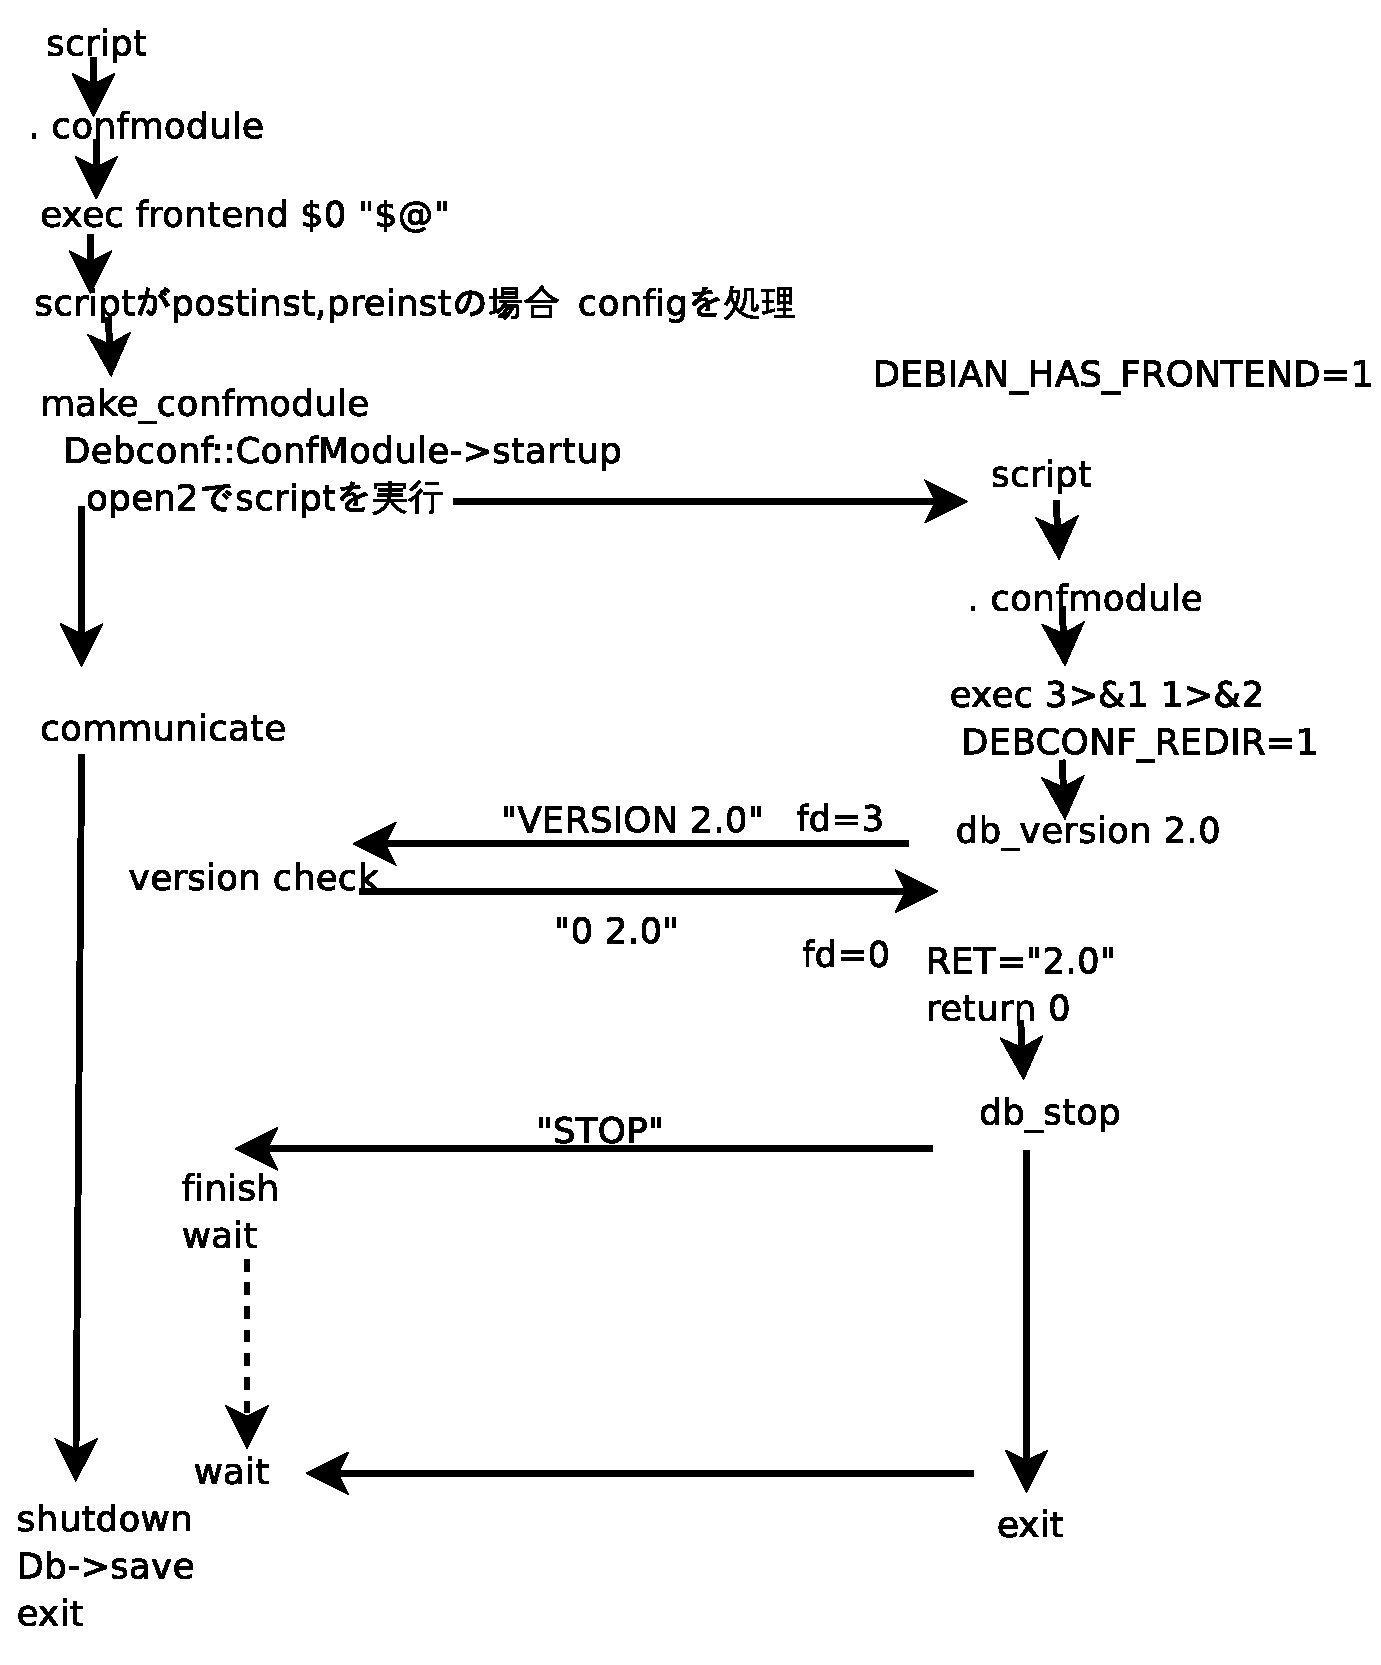
\includegraphics[scale=0.7]{image200509/debconf-protocol.eps}

\subsection{debconfデータベース}

debconfで設定したデータはどこにあるのでしょうか? この設定は/etc/debconf.confに記述されています。

デフォルトでは /var/cache/debconf に次のようなファイルとして格納されています。

\begin{table}[htbp]
 \begin{center}
 \begin{tabular}[htbp]{|l|p{20em}|}\hline
  ファイル名 & 内容 \\ \hline
  templates.dat & templatesの情報 \\ \hline
  config.dat & 設定データ \\ \hline
  password.dat & パスワードデータ \\ \hline
 \end{tabular}
 \end{center}
 \caption{debconfデータベース}
 \label{debconf:dbfile}
\end{table}

debconfデータベースの内容は debconf-get-selections を使うとダンプすることができます。この出力を debconf-set-selectionsの入力として渡すとロードすることができます。\footnote{debconf-get-selectionsは TABで分割していて、debconf-set-selectionsでは(特にタイプと値の間は)空白文字列一つだけという点に注意したほうがいいでしょう。ファイル経由でやりとりしたりパイプ経由の場合は問題ありませんが、ターミナルの出力をコピペするとはまることがあります(TABが複数のスペースになってしまっているので)}

debconf-get-selections --installerで、debian-installerで使ってdebconfデータベースをとりだすことができます。

その他に debconf-copydb を使うことでデータベースファイルをコピーすることができます。

\subsection{debconfを使っているスクリプトのデバッグ}

debconfを使ってるスクリプトのデバッグは簡単ではありません。しかし基本はDEBCONF\_DEBUGに値を設定してスクリプトを実行すればいい場合が多いでしょう。

\begin{commandline}
 # DEBCONF_DEBUG='.*' /var/lib/dpkg/info/パッケージ.postinst configure 最後に設定されたバージョン
\end{commandline}

これでパッケージの設定する時のdebconfの動きを追うことができます。なお簡単にするためにdpkg-reconfigure debconfでdebconfフロントエンドをReadlineなどをにしておいた方がいいでしょう。

DEBCONF\_DEBUG='.*'というのは DEBCONF\_DEBUG=user、DEBCONF\_DEBUG=developer、DEBCONF\_DEBUG=dbすべてを指定したのと同じ意味になります。

debconf-communicateを使うと、debconfデータベースと直接やりとりすることができます。標準入力からコマンドを与えると、標準出力に結果をかえします。コマンドはdebconfシェルモジュールでつかうコマンドからdb\_をとりのぞいたものになることに注意しましょう。例えば次のように使います。

\begin{commandline}
 # echo 'get debconf/priority' | debconf-communicate
 0 critical
\end{commandline}

0が成功を意味\footnote{db\_getの終了値}し、criticalがdebconf/priorityの値\footnote{db\_getを実行した場合だと\$RETに設定される値}を意味します。

\subsection{おわりに}

本文書ではDebianで設定データの管理を司っているdebconfについて解説しました。

\dancersection{apt-listbugs の生い立ちと実装}{樽石}
\label{sec:taruishi}
%% taruishiさんの記事はここから 
この文書は 2005 年 3 月に北京で開催された Asia Debian Mini-Conf
in Beijin で発表した資料の日本語訳です。

\subsection{はじめに}


Debian は 24 時間 365 日、多くの開発者によって日夜開発されている自由
なオペレーティングシステムです。わたしたちはこのような最新のスナップショットを
Debian のアップグレードフレームワークを使うことで簡単に共有することができ、
実際に、このフレームワークを利用して多くの人が最新の Debian スナップショット
を利用しています。

一方で、この最新スナップショットはときどき壊れることがあります。apt-listbugs
は、このような壊れたスナップショットからあなたのコンピュータを守るための仕組みです。

この短い文書では、apt-listbugs がどのようにコンピュータを守るのか、apt-listbugs
の生い立ち、実装について簡単に説明します。また apt-listbugs の抱えている
現在の問題点について紹介します。

\subsection{仕組み}

Debian には Debian バグ追跡システム(BTS) として知られる、Debian に関する
全ての問題が利用可能な中央管理型バグ追跡システムがあります。Debian のパッケージ
インストールフレームワークである APT は apt-get や aptitude 等を利用して
インストールやアップグレードを行う直前に BTS からこれらの問題を取得するために
apt-listbugs を呼び出します。apt-listbugs はどのパッケージがインストール
されるのか、またアップグレードされるのかを自動認識し、問題となるバグを見付けた場合は
その事をユーザに通知し、インストールを継続するか警告を出します。

このアプローチは、主にふたつの問題、ひとつはユーザの視点、もうひとつは開発者の視点
を解決します。

\subsubsection{ユーザの視点}

ユーザの視点は apt-listbugs のメインの目的です。APT フレームワークは
任意のパッケージを簡単にアップグレードすることができます。複雑な作業を
一切行わずに単に 'apt-get upgrade' と実行するだけです。これはすばらしい
機能ですが、一方でこのアプローチは壊れたパッケージさえも簡単にインストール
させてしまいます。多くの人が apt-get upgrade を利用しているため、
結果として世界中の Debian マシンが一瞬のうちに壊れてしまうことになります。

実際は、壊れたパッケージの情報は BTS に既に存在している可能性が非常に高いのですが
この情報が BTS にあるかどうかを毎回チェックしないといけないとしたら apt-get upgrade
による簡単なアップグレード作業は面倒な作業に一変してしまいます。これが
apt-listbugs が必要な理由です。apt-listbugs はそのような情報が BTS
にあるかどうかをあなたの代わりに毎回自動で行います。

\subsubsection{開発者の視点}

ふたつ目の目的は Debian 開発者のためのものです。基本的には、BTS は Debian
パッケージに関するあらゆる情報知るために利用できるすばらしいものです。もし
自分のパッケージにバグがあった場合、他のユーザが問題を BTS に報告してくれます。
開発者はいつでも、どこでも、この情報にアクセスすることができます。

しかし、仮に自分の環境ではたまたま発生しなかった致命的な問題が最新のパッケージ
に含まれてしまったとします。こうなると、多くのユーザは問題の深刻さを考慮して
急いでバグ報告をしようとします。それゆえ、たったひとつのバグに対して
非常にたくさんのバグ報告を受け取ることになってしまい、開発者はバグ報告の分類という
本質的でない作業に時間をとられ、本当に直したい致命的な問題の解決に長い時間
を要してしまうことになります。もし、ユーザがバグをレポートする前に似たような
レポートを閲覧することができれば、重複したレポートを送ることはなくなるでしょう。

\subsection{ヒストリ}

apt-listbugs はもともとユーザの視点をなんとかしたいという個人的な目的で
数年前に開発されました。ちょうどその時は、大学院を修了するために修士論文を
書かなければいけない時期でした。ところが、何を思ったか〆切の一週間前に
apt-get upgrade をしてしまったのです。結果、NFS が動かなくなり、この
問題を修正しなければいけなくなりました。このバグレポートをきちんとチェックして
いれば、このような問題にはあわなかったのですが、バグレポートを毎回チェック
するわけにはいきませんでした。なぜならいつインストールされるかわからない
致命的な問題のために毎回バグレポートをチェックするのは非常に大変な作業
だからです。

\subsubsection{CGI 問題}

apt-listbugs の最初のバージョンは Debian にすぐにアップロードすることは
できませんでした。その理由は apt-listbugs は BTS の CGI 出力を利用して
いたからです。CGI スクリプトはスクリプト言語で書かれていたため、もしこのパッケ
ージをアップロードすると、BTS サーバが非常に高負荷になってしまうことは容易に想像
できます。そこで、この apt-listbugs を利用したら同時にアクセスできるユーザ
数は何人程度なのか知るために CGI のパフォーマンスを測定することにしました。
結果は、1 パッケージのレポートを取得するのにかかる時間は約 1 秒でした。
BTS サーバは 2 台の CPU を備えていましたので、結局 1 秒に 2 つの
バグレポートしか取得できません。そのため、もし 10 個のパッケージをアップグレード
しようとしたら、レポートの取得に 5 秒かかってしまいます。これは非常に大きな
問題です。特に、BTS サーバは Debian のマスタサーバでしたから、もし Debian
ユーザ全員がそのサーバからバグレポートを取得したら、これはほとんど DoS アタック
のような状態に陥ってしまいます。

\subsubsection{強制キャッシュ}

最初に考えた解決法は CGI 出力のキャッシュを行うプロクシサーバを利用することでした。
プロキシサーバが http の No-Cache 属性を無視すれば、静的なデータを利用することが
できます。もちろん TTL の問題はありますが、DoS になってしまうよりは良いでしょう。

このサーバを用意したことで、とりあえず Debian に apt-listbugs をアップロード
することができましたが、はじめは experimental にアップロードして様子を見ていま
した。

\subsubsection{index.db パーサ}

はじめのバージョンの apt-listbugs はパーサに潜在的な問題を抱えていました。それは
パーサが CGI 出力を利用していたことです。CGI のフォーマットはドキュメント化されて
いません。また、CGI スクリプト自体遅いという問題もあります。そのため、別の
新しいパーサが必要でした。これは index.db パーサと呼ばれるパーサです。index.db
パーサは BTS の内部データベースである index.db ファイルを直接パースするパーサ
です。index.db ファイル自体もドキュメント化はされていないのですが、このファイルは
静的に生成されるものですので、CGI よりはずっと良い解です。

実際には、このパーサは index.db ファイルを critical や grave といった重要度毎
に分割した index.db ファイルを利用します。

\begin{center}
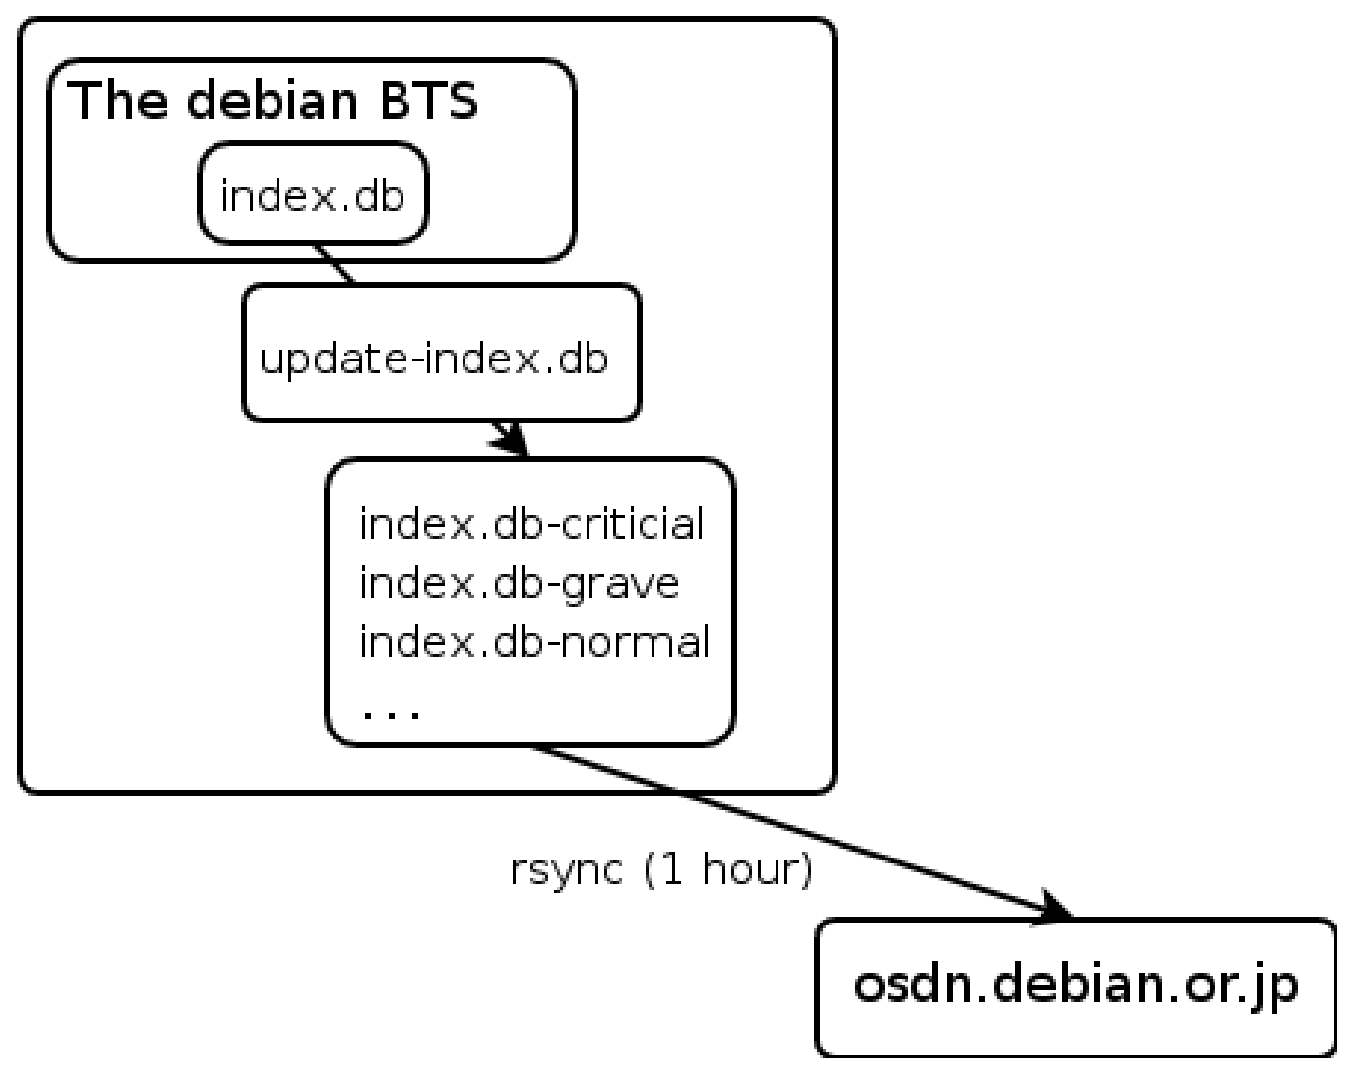
\includegraphics[scale=0.3]{image200510/indexdb.eps}
\end{center}

apt-listbugs には LDAP プロトコルを利用した実験的な LDAP パーサも存在しますが、
このパーサは CGI パーサの代わりにするには意味がないものでした。その理由は当時の
BTS LDAP サーバは内部的に tcl スクリプトを毎回よんでいるものだったからです。
速度に変化はありませんでした。

\begin{quote}
Andreas Barth 氏は BTS 用のネイティブな LDAP インタフェースを作成しました。
そのため、現在ではこのインタフェースを利用してバグを取得することが可能になっています。
詳細は \url{http://people.debian.org/~aba/bts2/ldap/} を参照してください。
ただ、このインタフェースを利用するインタフェースはまだ実装されていません。
\end{quote}

\subsubsection{SpamAssasin と apt-listbugs}

Index.db パーサを利用することで、apt-listbugs は動的なデータをサーバから
取得することはなくなりました。そこで、この時点で一時的な解決であった強制キャッシュ
サーバを停止しました。

しかし、これは別の問題を生み出したのです。ちょうどその頃、BTS に対して非常に
多くの SPAM メールが送られるようになっており、spamassasin が BTS サーバの
CPU を非常に多く使うようになっていたのです。そして CPU 大量消費の原因が
apt-listbugs にあるという勘違いされてしまったのです(Bug\#207415)。

よく考えてみると、1 日で 46,000 個の静的データが負荷をこれほどあげるはずは
ありません。秒に換算すればわずか 0.5 個のだからです。通常の Web サイトは
もっと多くの要求を処理できています。データサイズに関してはどうでしょうか。
ひとつのデータは約 100 バイトですから、これも 50B/s 程度です。いずれにしても
この問題の対策として apt-listbugs はサーバへの直接アクセスを禁止されて
しまいました。

とはいえ、この問題が apt-listbugs によるものであったとしてもなかったとしても
apt-listbugs がマスタサーバに直接アクセスするのはあまり良い考えではありません。
そこでこの問題をきっかけに osdn.debian.or.jp にミラーサーバを構築しました。

現在、1 日に 4500 システムが apt-listbugs を使用しています。以下のグラフは
どれくらいの Debian システムが apt-listbugs を利用しているかを表しています。
X 軸は osdn.debian.or.jp にミラーサイトを構築した日からの日数、Y 軸は
1 日に osdn.debian.or.jp にアクセスする IP アドレスの数です。

\begin{center}
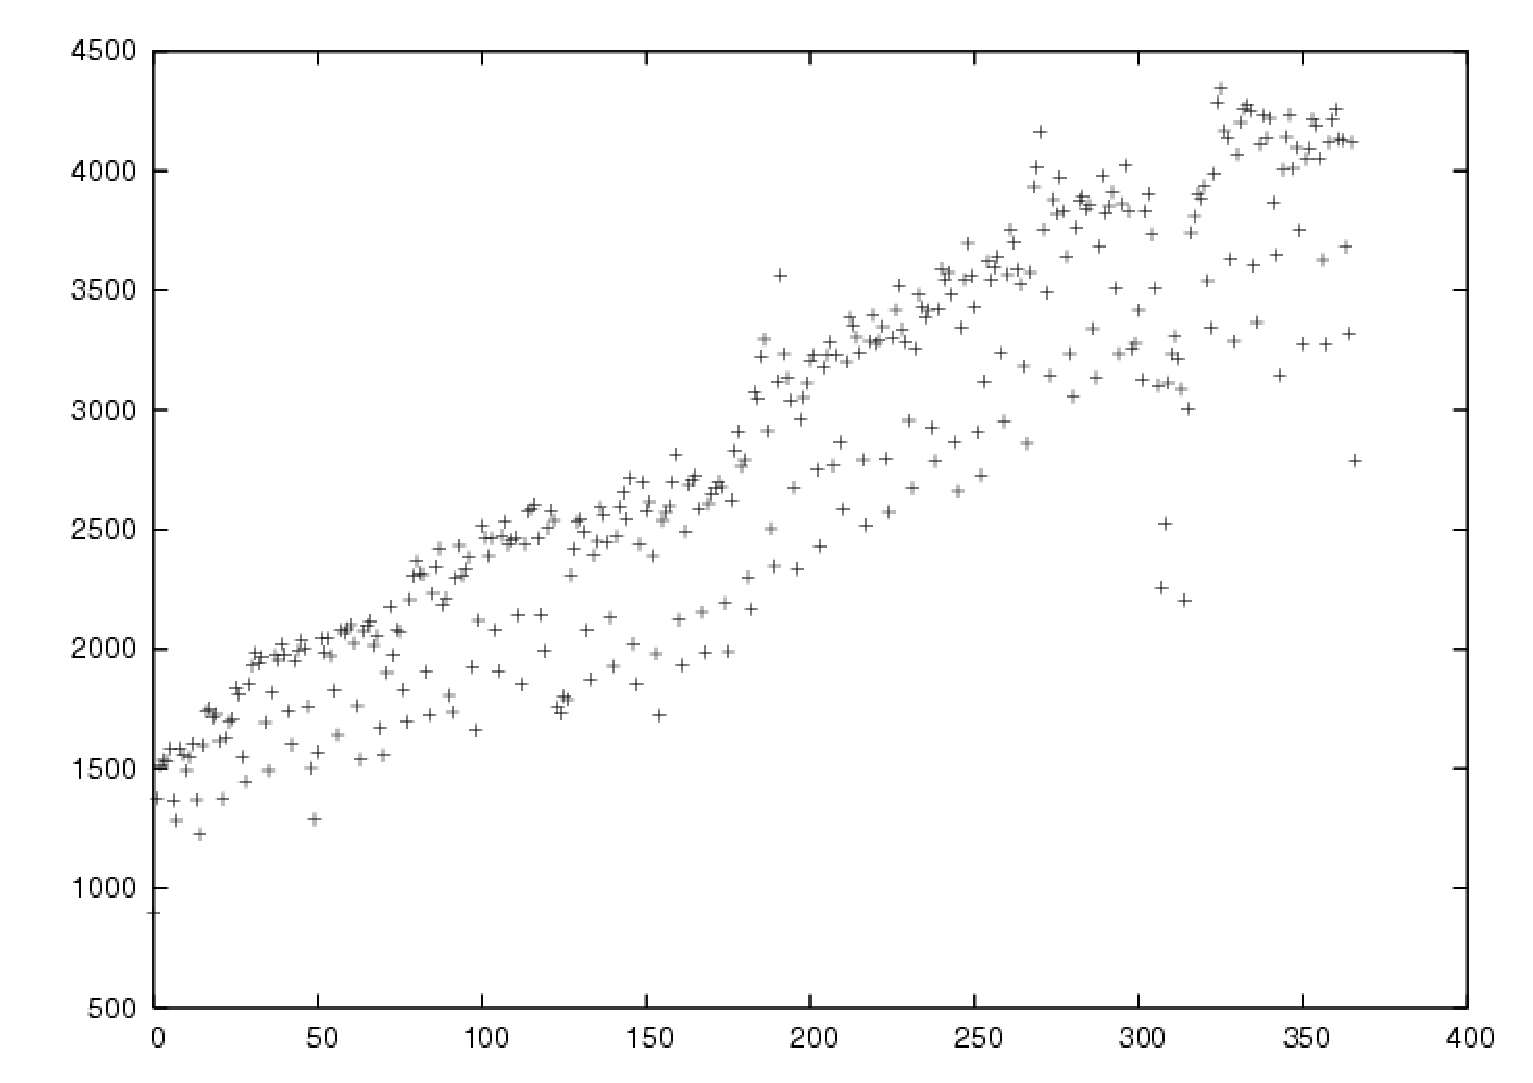
\includegraphics[scale=0.5]{image200510/user.eps}
\end{center}

\subsection{実装}

apt-listbugs は オブジェクト指向スクリプト言語のひとつである Ruby で記述されています。
主に以下のクラスから構成されています。

\begin{verbatim}
* Acquire
 * HTTP
 * File
* Parser
 * CGI
 * Index
 * DSA
 * ReleaseCritical
* Bug
* Factory
 * PackageFactory
 * StatusFactory
 * BugsFactory
* Viewer
 * SimpleViewer
 * RSSViewer
\end{verbatim}

\subsubsection{Acquire}

Acquire はデータを取得するクラスです。このクラスはサブクラスに対するキャッシュ機構
を実装しています。実際の取得メソッド実装されておらず、サブクラスで実装します。
例えば、HTTP サブクラスはデータを http から取得し、File サブクラスはデータを
ファイルシステムから取得します。

\subsubsection{Parser}

Parser クラスは Acquire クラスで取得されたデータをパースし、バグ情報を保持する
Bugs クラスを生成します。例えば以下の ruby コードは CGI 出力から apt-listbugs
のバグ情を取得します。

\begin{verbatim}
acq = Debian::BTS::Acquire::HTTP.new
cgi_parser = Debian::BTS::Parser::CGI.new(acq)
bugs = cgi_parser.parse("apt-listbugs")
bugs.each do |bug|
  p bug
end
\end{verbatim}

- CGI

 CGI パーサは bugs.debian.org から取得した CGI 出力をパースします。

- Index

 Index パーサは BTS システムの生データである index.db ファイルをパースします。
 apt-listbugs のデフォルトパーサです。

- DSA

 DSA パーサは Debian セキュリティアドバイザリのページをパースします。

- ReleaseCritical

 ReleaseCritical は Release-Critical ページをパースします。

\subsubsection{Bug}

 Bug クラスは ID、題名、重要度、タグ等のバグ情報を保持します。

これらのクラスは汎用的に作成されています。そのため、apt-listbugs 以外の
プログラムからでもこれらのクラスを利用することが可能です。

\subsubsection{Factory}

Factory クラスは「仕様書」からインスタンスを生成します。実際の作成は
サブクラスにより行われます。このクラスは進捗表示等の Factory に汎用的な
メソッドのみを実装しています。

- PackageFactory

PackageFactory は .deb ファイルの一覧からパッケージ情報を生成します。

\begin{verbatim}
# creating new packages database
new_pkgs = Factory::PackageFactory.create(pkgnames) do |msg, val|
  config.frontend.progress(msg, val) if config.quiet == false
end
Factory::PackageFactory.delete_ignore_pkgs(new_pkgs)
\end{verbatim}

この処理が行われている間は、apt-listbugs から以下のメッセージが出力されます。

\begin{verbatim}
パッケージフィールドを読み込んでいます...
\end{verbatim}

- StatusFactory

StatusFactory は指定したパッケージ名に対するの現在のシステムの情報を取得します。
この処理中は以下のメッセージが出力されます。

\begin{verbatim}
パッケージ状態を読み込んでいます...
\end{verbatim}

- BugsFactory

BugsFactory は Bug クラスで表現されるバグ情報を生成します。基本的に、この
Factory はパーサクラスの単なるラッパーですが、パーサクラスは一度にひとつの
パッケージのみを処理するのに対し、BugsFactory は複数のパッケージを処理できます。

\begin{verbatim}
バグレポートを取得しています...
\end{verbatim}

\subsubsection{Viewer}

Viewer クラスはバグを表示するビューアを提供します。

- SimpleViewer

SimpleViewer は以下のような処理を行う組み込みの対話的ビューアです。

\begin{verbatim}
critical bugs of cron (3.0pl1-86 -> 3.0pl1-87) <done>
 #282722 - Network install of Debian Woody Alpha -  cron corrupt on debian servers ?
grave bugs of strace (4.5.8-1.2 -> 4.5.9-1) <done>
 #294172 - strace - builds no s390 binary
grave bugs of gaim (1:1.1.2-3 -> 1:1.1.3-1) <done>
 #295904 - gaim: 1.1.3-1:  dies with SIGABRT on startup
grave bugs of reportbug (3.7.1 -> 3.8) <done>
 #295853 - reportbug includes sensitive information in report
grave bugs of cdbs (0.4.26-4 -> 0.4.27-1) <open>
 #295884 - cdbs: Changes control file to add new build dependency.
grave bugs of libdb4.3 (4.3.27-1 -> 4.3.27-2) <open>
 #294163 - libdb4.3: build failed on hppa
Summary:
 strace(1 bug), gaim(1 bug), cron(1 bug), cdbs(1 bug), libdb4.3(1 bug), reportbug(1 bug)
Are you sure you want to install/upgrade the above packages? [Y/n/?/...]
\end{verbatim}

- RSSViewer

RSSViewer はバグ情報を RSS (Really Simple Syndication) 形式で出力します。

\begin{center}
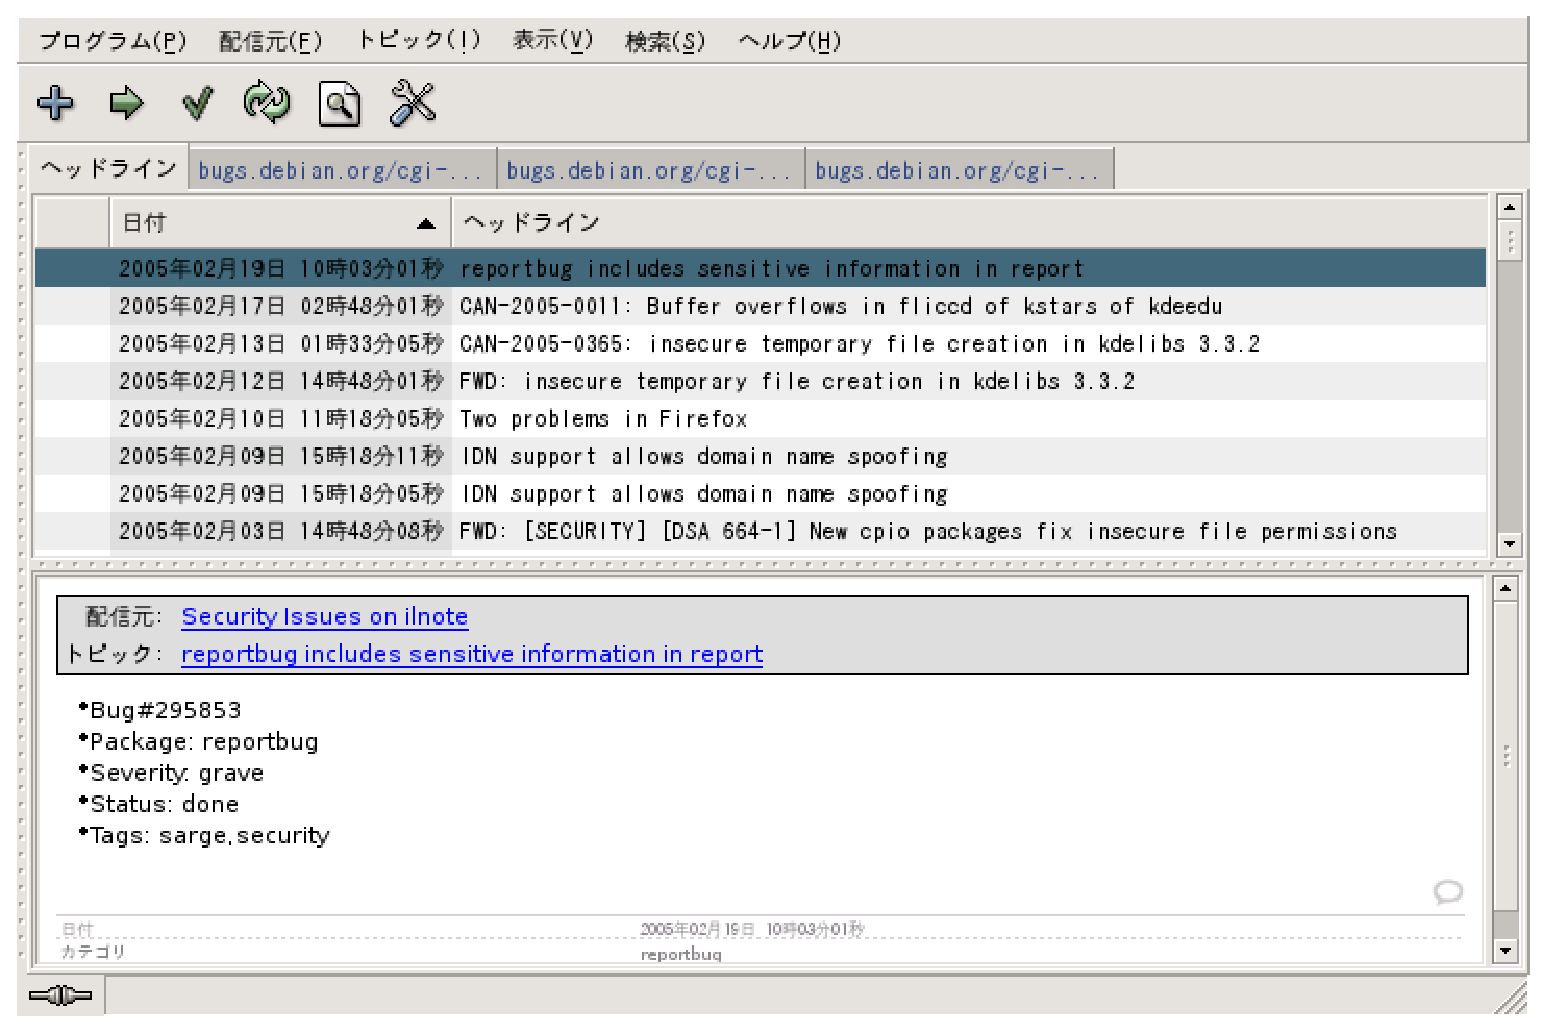
\includegraphics[scale=0.5]{image200510/rss.eps}
\end{center}

\subsection{問題}

現在、apt-listbugs が抱える一番の問題点は、apt-get upgrade を行うたびに
apt-listbugs が大量のバグを表示してしまうことです。しかもほとんど役に立たない
多くのレポートを読まなければいけません。それはそれほど重要でもない問題を重要だ
とタグ付けされた報告が非常に多いことが原因です。apt-listbugs は changelog
ファイル中の ''closes: Bug\#XXXX'' という形式の文字列を処理することで
不要なレポートを表示しないようにしていますが、上記のようなレポートはパッケージ
保守担当者によって手動でクローズされてしまうため、表示から取り除くことはできません。

バグには open, done 等の状態があるのですが、これを使うことはできません。
それはバグの状態というのは終局的なシステムだからです。バグ報告は通常そのバグを
修正した新しいパッケージが Debian にアップロードされるとすぐにクローズされます。
この段階では、バグ状態は変更されますが、そのバグを修正したパッケージはまだ
利用できません。ミラーサイト使っている場合、この遅延時間もっと長くなるでしょう。

最初のバージョンの apt-listbugs はレポート文書中に存在する ``Version'' タグ
を利用しており、これによりいくつかのバグをフィルタすることができていました。この
情報を利用すると

\begin{itemize}
\item 既にバグが存在している
\item インストールしようとしているバージョンとは関係がない
\end{itemize}

といったフィルタリングが可能でした。しかし、現在は apt-listbugs が
CGI にアクセスできないため、この情報を利用することができません。おそらく
Since や Fixed-In といったような汎用的なタグ情報が必要であると
考えています。

\subsection{Tips}

apt-listbugs はいろいろな利用方法があるためここでいくつか紹介します。

\subsubsection{RSS によるセキュリティ問題}

\begin{verbatim}

dpkg --get-selections | grep -v deinstall | awk -F' ' '{print $1;}' | \
   xargs -n $num /usr/sbin/apt-listbugs -y -q -T security --title \
   "Security Issues on `hostname --fqdn`" rss
\end{verbatim}

このスクリプトは /usr/share/doc/apt-listbugs/security にあります。

\subsubsection{作業中のパッケージで解決していないバグを見る}

\begin{verbatim}

grep -e ^Package:  < debian/control  | cut -d' ' -f2- | \
  xargs /usr/sbin/apt-listbugs -S outstanding,open \
    critical,grave,serious,important,normal,wishlist,minor list
\end{verbatim}

このスクリプトは /usr/share/doc/apt-listbugs/deblistbugs にあります。

\subsection{まとめ}

apt-listbugs はまだいろいろ問題を抱えていますが、基本的な概念は非常におもしろい
ものです。現在の興味は apt-listbugs に webrick 等を使って組み込み http サーバ
を導入することです。このフロントエンドを利用すると apt-listbugs の管理が非常に
便利になります。また、bts2ldap を利用した LDAP バックエンドも必要であると考えています。

\subsection{参考}

\begin{itemize}
\item Debian - \url{http://debian.org/}
\item Debian Bug Tracking System - \url{http://bugs.debian.org/}
\item \url{http://lists.debian.org/debian-devel/2003/08/msg02376.html}
\end{itemize}

%% end

\dancersection{``claim'' makes Debian better}
{やまね}
\label{sec:yamane}
%%yamaneさんの記事はここから

\subsection{本日の目的}

Debian BTSについて理解を深める

\begin{itemize}
\item BTSって何さ?
\item どういうときにするの?
\item 何がいいの?
\item 実際どうすればいいの?
\end{itemize}

そして立派なクレーマーとして認められる!

\subsection{Debian Bug Tracking System}

Debian独自のバグ追跡システム。
システムとしてはdebbugsという独自のものを利用

\subsubsection*{特徴}

\begin{itemize}
\item Webから閲覧可能(まぁ、最近のは皆そうですね)
\item やり取りは基本的に全てオープン
\item メールベースで作業が進む(ここは珍しいかも)
\item かなり使い込まれてます。30万件近くが登録済み。\\
redhatのbugzillaはこの半分ぐらいの件数
\end{itemize}

\begin{figure}[htbp]
\begin{center}
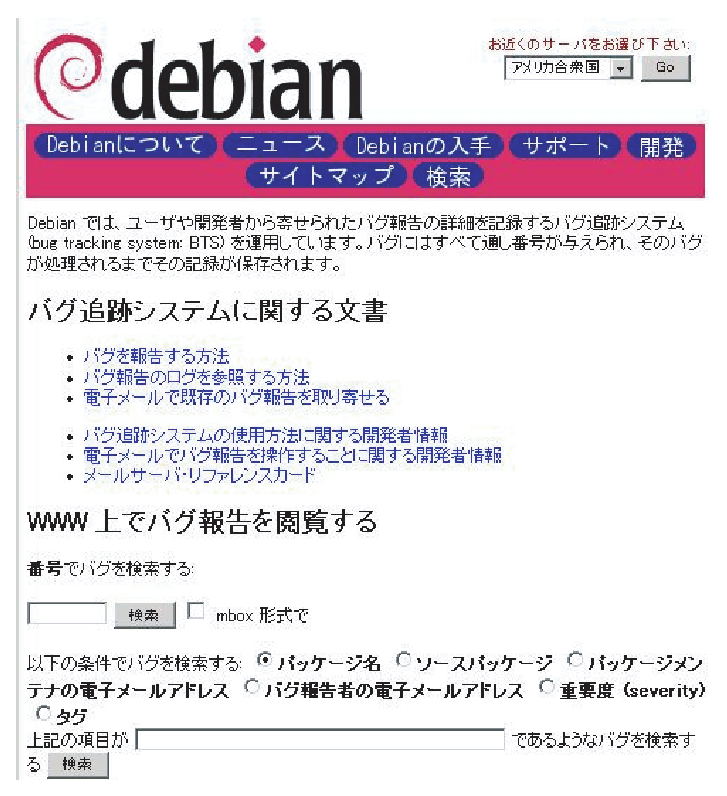
\includegraphics{image200508/bts.eps}
\end{center}
\caption{BTSのページ(http://www.debian.org/Bugs/)}
\label{bts-webpage}
\end{figure}

\subsubsection{どんなときにBTSを利用しますか?}

\begin{itemize}
\item パッケージングのバグに遭遇したとき
\item アップグレードしたらよくわからない現象が起こるようになってしまったとき
\item いつまで経ってもsecurity fixが提供されないとき
\item 気の利いた機能を実装したのでパッチを取り込んでもらいたいとき
\item 地味〜なL10Nな作業を取り込んでもらうとき
\item セキュリティホールの報告があったのでメンテナをせっつきたいとき
\end{itemize}

\subsubsection{擬似パッケージ (pseudo package)}

パッケージではないが、BTSで扱うためにパッケージとして扱うもの

\begin{itemize}
\item Webサイト
\item wnpp -- 作業が望まれるパッケージ(ITPも)
\item インストールシステム	などなど
\end{itemize}

\url{http://www.debian.org/Bugs/pseudo-packages.ja.html}参照

\subsubsection*{ここでのポイント}

あらゆる苦情・提案はBTSに集まる。誰も聞いていないところで文句を言うのではなくBTSすべし。

\subsection{BTS用ツール}

\subsubsection{reportbug/querybts}

\subsubsection*{reportbugコマンド}

簡単にバグレポート・レポートの検索が可能

\begin{itemize}
\item 対話的な操作が可能です。
\item レポートはメールで飛びます。ポーンと。
\item レポートはgnupgで署名も可能。まるでちゃんとした報告みたいに見えます。
\end{itemize}

\begin{figure}[htbp]
\begin{center}
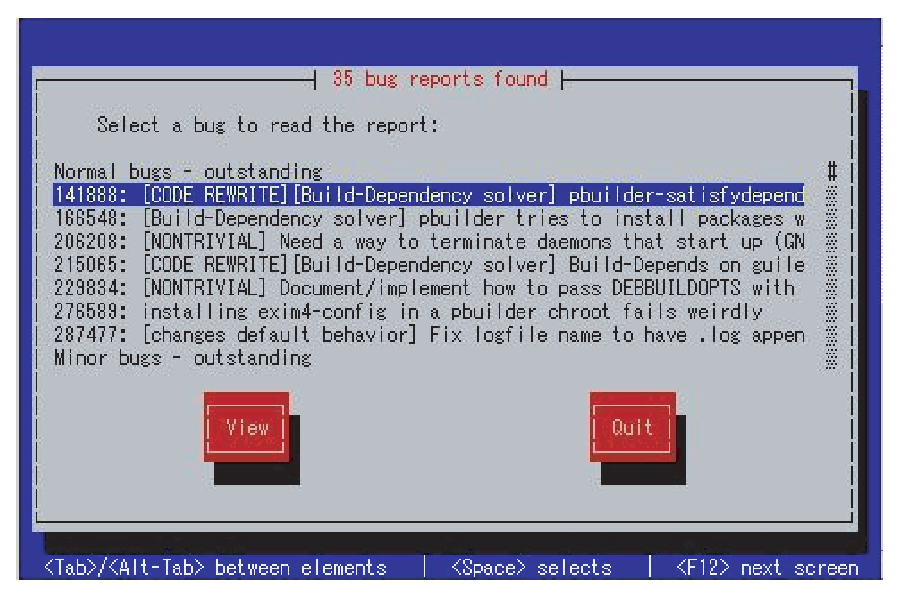
\includegraphics{image200508/reportbug.eps}
\end{center}
\caption{reportbugの画面}
\label{reportbug}
\end{figure}

\subsubsection*{querybtsコマンド}

バグレポートの検索に特化しています。

\subsubsection{debbugs-el}

emacs ユーザは、 debbugs-el パッケージに含まれる debian-bug コマンドを使うこともできます。M-x debian-bug と入力すると、reportbug とよく似たやり方で、全ての必要事項を尋ねられます…らしい。(emacs使ってないので不明)

\subsection{「重要度」と「タグ」}

\subsubsection{Severity (重要度) レベル}

\url{http://www.debian.org/Bugs/Developer#severities}参照

\begin{itemize}
\item critical(致命的)

システム上の関係のないソフトウェア (またはシステム全体) を破壊する、重大なデータの欠落を引き起こす、または、そのパッケージをインストールしたシステム上でセキュリティホールが生じる場合。 

\item grave(重大)

問題のあるパッケージが使用できない、またはほとんど使用できない。またはデータの欠落を引き起こす、そのパッケージを使用するユーザのアカウントにアクセスを許してしまうセキュリティホールが生じる場合。 

\item serious(深刻)

Debian ポリシーに対して見すごせない違反がある (大まかに言うと、"must" や "required" の要件に違反している)、またはパッケージメンテナの意見としてそのパッケージがリリースに適していないと判断された場合。 

\item important(重要)

バグがパッケージの利用に大きく影響しており、対処しなければ誰にもまったく使用できない場合。 

\item normal(通常)

デフォルト値。通常のバグ。 

\item minor(軽度)

問題がパッケージの利用に影響しない、かつ修正はたいした事がないと思われる場合。 

\item wishlist(要望)

将来的な要望、主に設計上の理由により修正が非常に困難なバグ。
\end{itemize}

\subsubsection{タグ}

\url{http://www.debian.org/Bugs/Developer#tags}参照

\begin{itemize}
\item patch(パッチ)

バグ報告に、バグを修正するためのパッチや簡単な手順が含まれています。 パッチがあってもバグを適切に解決できない場合や別の問題を生じる場合は、 このタグは使うべきではありません。 

\item security(セキュリティ)

このバグはパッケージのセキュリティ問題を説明します。 ほとんどのセキュリティバグは、critical (致命的) や grave (重大) の severity (重要度) も設定すべきです。 

\item upstream(上流)

このバグは、パッケージの上流の部分に影響します。

\item d-i(インストーラ)

 このバグは、debian-installer に関するものです。 インストーラの開発に関係するけれども、インストーラの直接の 構成要素ではないパッケージに対するバグの場合、このタグを使ってください。 

\item L10n

このバグは、パッケージの地域化に関するものです。 

\item woody / sarge / sid / experimental

このバグは特に各ディストリビューション に加えられるものです。
\end{itemize}

\subsection{BTSの心得}

\begin{itemize}
\item 何よりも相手を尊重しよう
\item 事実を端的に述べよう
\begin{itemize}
\item 環境の記述は多すぎず少なすぎずを目指そう
\item バージョンやアーキテクチャぐらい書こう(面倒な人はツールを使いましょう)
\end{itemize}
\item broken English でもいいや、と開き直ろう
\item でも多少は体裁は整えておこう
\begin{itemize}
\item gnupg 使ってみるとか
\item 定型シグネチャ使っておくとか
\end{itemize}
\end{itemize}

\dancersection{Starting debconf translation}
{やまね}

\url{http://kmuto.jp/debian/po-trans/}に翻訳の状況が掲載されている。

\subsection{必要なもの}

\begin{itemize}
\item debconf-updatepo

poが最新のものかをチェック

\item msgfmt

文法があっているかをチェック
\end{itemize}

\subsection{手順}

\begin{enumerate}
\item po-debconfをインストール

\begin{commandline}
apt-get install po-debconf
\end{commandline}

\item 翻訳したいパッケージのソースをインストール

\begin{commandline}
apt-get source <packagename>
\end{commandline}

\item template.poをコピーして翻訳する

\begin{commandline}
cd <packagename>/debian/po
cp template.pot ja.po
\end{commandline}

\item 査読してもらう

debian-doc@debian.or.jpとかに投げる

\item BTSする

\begin{commandline}
reportbug -A 翻訳したファイル -g
ファイルを添付してGPG Signしてバグレポート送信
\end{commandline}

\end{enumerate}

%%ここまで

\dancersection{debbugs internal}{上川}
\label{sec:uekawa}
\subsection{はじめに}

この文書は Anthony Towns が フィンランドの debconf 5 で発表した内容を
日本にて展開するための資料です。
Anthony Townsの作成した英語の資料を省略して抜粋しています。
また、それ以降に変更した事項について追記しています。

Debian Bug Tracking System (BTS)は、ほぼDebianに特化したバグ報告の管理
のためのシステムです。
他のプロジェクトでも利用されていることもありますが、Debianでバグがパッケージベー
スで厳格に分類できることなどの特性が反映されているため、Debianプロジェク
トのワークフローで使いやすいように作られています。
\footnote{Debian のインフラと統合されており、changelogにバグ番号を記述してパッケー
ジをアップロードしたらバグが修正されたと記録されるようになっていたりします。}

規模としては、55000以上の現在アクティブなバグ報告、
231000のアーカイブされたバグ報告を現在保持していて、
毎週1000以上の新規のバグ報告が追加されています。
ウェブインタフェースは追加された報告をすぐに反映しており、
過去、ダウンタイムもほとんど発生していません。

Anthony Townsによると下記がバグトラッキングシステムの要件です。

\begin{itemize}
 \item インタフェース: 開発者がメールで操作できるようになっており、誰で
       もウェブで閲覧できるようになっている。
 \item パッケージベース: バグ報告をパッケージ別に高速に管理する必要があ
       る
 \item スケーラビリティー: 大量のバグ報告に対応できる必要がある
 \item 即時性: 現在のバグの状態をすぐに報告してくれる必要があり、バグの
       状態が変更されたらすぐに反映される必要がある
 \item 安定性: 継続して動作する必要がある。新規の機能がどんどん追加さ
       れたとしても。
 \item 公開: 議論の内容にDebianコミュニティー全体として参加できるように、
       永続的な公開記録として保存される必要がある。
\end{itemize}

\subsection{データ形式}

バグデータベースのスプールの形式は下記です。
リレーショナルデータベースなどは利用していません、
スプールディレクトリ以下にほとんどのデータが格納されています。

各バグについて、ファイルはそれぞれ
4個あります。
サマリーファイルはメタデータを保存します。
ログファイルは、そのバグに対して流れたメールを全て保存します。

statusファイルは互換性のためだけに存在しています。
reportファイルは、最初のバグ報告のメールで、バグが close されるときに送
信されるものです。

\begin{itemize}
 \item /org/bugs.debian.org/spool
       \begin{itemize}
	\item incoming/
	      \begin{itemize}
	       \item T.*
	       \item S[BMQFDU RC] *.*
	       \item R[BMQFDU RC] *.*
	       \item I[BMQFDU RC] *.*
	       \item G[BMQFDU RC] *.*
	       \item P[BMQFDU RC] *.*
	      \end{itemize}
	\item db-h/
	      \begin{itemize}
	       \item 00/
		     \begin{itemize}
		      \item ..
		      \item 314200.log
		      \item 314200.report
		      \item 314200.status
		      \item 314200.summary
		     \end{itemize}
	       \item ..
	       \item 99/
	      \end{itemize}
	\item archive/
	      \begin{itemize}
	       \item 00/
	       \item ..
	       \item 99/
	      \end{itemize}
	\item index.db -- index.db.realtimeへのシンボリックリンク
	\item index.archive -- index.archive.realtimeへのシンボリックリ
	      ンク
	\item nextnumber
       \end{itemize}
\end{itemize}

\subsubsection{incoming}

incomingに来たメールは処理中、名前を変えます。

\begin{itemize}
 \item T receiveによってうけとられた
 \item S SPAM確認待ち
 \item R SPAM確認中
 \item I SPAMチェック通った
 \item G service か process スクリプトを通った
 \item P process中
\end{itemize}

また、ファイル名の二つ目の文字はどこのメールアドレスにメールが送信されて
きたものなのかということを示します。
ファイル名ののこりは、バグ番号と、一意なIDです。
一意なIDを決定するのに現在は時間とプロセス番号を利用しています。

\begin{itemize}
 \item B: 通常のバグ報告。submit@ 1234@
 \item M: -maintonly メーリングリストに投げない
 \item Q: BTSに登録しない。-quiet
 \item F: アップストリームにフォーワード -forwarded
 \item D: バグ終了 -done
 \item U: サブミッターにメール -submitter
 \item R: ユーザのリクエスト用インタフェース request@
 \item C: デベロッパーの制御用インタフェース control@
\end{itemize}

\subsubsection{StatusとSummary}

statusファイルの中身は行ベースです。
無い行については空行とみなします。
このファイルは今後なくしていこうとしています。

\begin{itemize}
 \item バグ報告者のメールアドレス
 \item 時間(秒)
 \item サブジェクト
 \item 元のメールのメッセージID
 \item バグがアサインされているパッケージ
 \item タグ
 \item closeした人のメールアドレス
 \item 上流のメールアドレスかURL(forwardされたばあい)
 \item マージされているバグ番号
 \item severity
\end{itemize}

summary ファイルはRFC822形式で、拡張可能になっています。
現在Format-Version: 2 と 3 の二つの形式があります。
3は、ヘッダについてはRFC1522(MIME)のデコードされた形式になっています。

\begin{itemize}
 \item Format-Version: このファイル形式のバージョン
 \item Submitter: バグ報告者のメールアドレス
 \item Date: 時間(秒)
 \item Subject: サブジェクト
 \item Message-ID: 元のメールのメッセージID
 \item Package: バグがアサインされているパッケージ
 \item Tags: タグ
 \item Done: closeした人のメールアドレス
 \item Forwarded-To: 上流のメールアドレスかURL(forwardされたばあい)
 \item Merged-With: マージされているバグ番号
 \item Severity: severity
 \item Owner: バグの所有者
\end{itemize}

\subsubsection{logファイル}

あらゆるメールがlogファイルには追記されていきます。
また、メタデータも追記されていきます。
残念ながら、メタデータは生のHTMLで書かれており、
またバージョンによって記述の仕方が変わっており、
さらに悪いことに、古いバグの中にあるテキストは更新されていないため、
機械的に処理することは難しくなっています。

また、コントロール情報は、行頭のエスケープコードにより切り替わります。
メールの中にエスケープコードのような文字列が出て来たら、それは
文字コード030(8進数)の文字を追加してエスケープします。

詳細はDebbugs::Logを見てください。

\begin{itemize}
 \item kill-init: まだ一行も処理していません
 \item incoming-recv: 07: あとにgoがくる、Received:行
 \item autocheck: 01: X-Debian-Bugs-..: までの無視されている行、
       autowaitが次に来る
 \item html: 06: 生で表示すべきHTML
 \item recips: 02: メールの受取人、04で分割されている
 \item go: 05: メールの文書
 \item go-nox: X: メールの文書、Xではじまる行
 \item kill-end: 03: メッセージの終り。
 \item autowait: go-noxがあとにくる、空行まで無視されるその他の情報。
\end{itemize}

\subsubsection{Indexファイル}

indexファイルは、pkgreport.cgiがどのパッケージにどのバグがわりあてられて
いるかを確認するための情報です。

以前は、by-package.idxとby-severity.idxというのがあり、高速化に貢献する
はずだったのですが、
一年以上長い間生成されていなかったうえに、生成されていなかったことに
誰も気づかなかったので必要ないんじゃないだろうか、ということです。

データ形式としては下記のようになります。
パッケージ、バグ番号、時間、ステータス、メールアドレス、severityの順に書
いた行が全てのバグに対して作成されています。

\begin{commandline}
 pbuilder 317998 1121196782 open [Junichi Uekawa <dancer@netfort.gr.jp>] normal
\end{commandline}

\subsection{コード形式}

debbugsは特に設計もされずに長い間パッチを累積してきました。
ただ、明確にわかれている部分はあって、メールを処理するコアのインタフェー
スのスクリプトと、
ウェブを表示するためのCGI部分とで分離できます。

設定ファイルは全て/etc/debbugs にあります。

\subsubsection{コアのスクリプト}

メールを処理する部分があります。

\begin{itemize}
 \item errorlib: ライブラリ
 \item receive: MTAからメールを受信する
 \item spamscan: 受信メールをSPAMチェックする
 \item processall: process と service にメールを分配する
 \item process: バグメールを処理する
 \item service: control@ と report@ メールを処理
 \item expire: closeされてから28日過ぎたバグをエキスパイア処理する
 \item rebuild: indexファイルをリビルド
\end{itemize}

receive と rebuild 以外は cronから起動しています。
15分に一回しか動作しません。

\subsubsection{CGIスクリプト}

CGI関連は、
errorlib関数を活用している部分もありますが、ほぼ独立しています。

\begin{itemize}
 \item bugreport.cgi: バグレポートを一つ表示
 \item pkgreport.cgi: パッケージやサブミッタなどでサマリを作成する
 \item pkgindex.cgi: パッケージやseverityに対して数を表示
 \item common.pl: ライブラリとして利用
\end{itemize}

pkgreport.cgiはユーザが直接ウェブでたたくため、
特に速度が重要視される部分なので、触る場合には注意してください。

\subsubsection{ハックするには}

debbugsのソースはCVSにあります。
また、Debian Developerであれば、
ミラーが merkel.debian.orgの/org/bugs.debian.org以下にあります。

\subsection{そして何がおきたか}

Anthony Townsの発表でどういう結果がもたらされたか見てみましょう。

\subsubsection{バージョントラッキング}

バグがどのバージョンで発見され、どのバージョンで修正されたのかというのを
トラッキングできるようになりました。
従来は発見されたバージョンだけがVersionヘッダで分かるようになったのです
が、それ以外の情報も保持するようになりました。

\url{http://lists.debian.org/debian-devel-announce/2005/07/msg00010.html}

バグ番号を保持して操作するためのBTSのコマンドは下記です。

\begin{commandline}
close バグ番号 バージョン
reassign バグ番号 パッケージ バージョン
found バグ番号 バージョン 
\end{commandline}

また、katieが変更され、バグをcloseするメッセージには、下記のヘッダが付くよう
になりました。それをBTSが処理してcloseされたバージョンを把握できるように
なりました。

\begin{commandline}
 Source-Version: バグ番号
\end{commandline}

CGIに対して、versionを指定すると、そのバージョンでの状態がでてきます。
\debianbug{329344}は、0.4ではopenだったが、0.5ではcloseになったというの
が
\url{http://bugs.debian.org/cgi-bin/pkgreport.cgi?pkg=cowdancer&version=0.4}と
\url{http://bugs.debian.org/cgi-bin/pkgreport.cgi?pkg=cowdancer&version=0.5}
二つのページを比較するとわかります。

/org/bugs.debian.org/spool/db-h/44/329344.summary
を見ると、メタデータとして保存されているのがわかります。

\begin{commandline}
Format-Version: 2
Found-In: cowdancer/0.4
Done: Junichi Uekawa <dancer@debian.org>
Subject: cowdancer: cow-shell does not start, gives error
Date: 1127295198
Submitter: Francesco Potorti` <Potorti@isti.cnr.it>
Fixed-In: cowdancer/0.5
Package: cowdancer
Message-Id: <E1EI0YD-0003lE-00@pot.isti.cnr.it>
Severity: grave
\end{commandline}

\subsubsection{ユーザタグ}

\url{http://lists.debian.org/debian-devel-announce/2005/09/msg00002.html}

request@bugs.debian.orgに対して下記のようなメールをおくればタグが追加で
きます。

\begin{commandline}
    user aj@azure.humbug.org.au
    usertag 18733 + good-reasons-to-run-for-dpl
    usertag 18733 + still-cant-believe-it-finally-got-fixed
    usertag 62529 + your-days-are-numbered
\end{commandline}

見る際には、
users=でユーザを指定するとタグが見えるようになります。

\url{http://bugs.debian.org/cgi-bin/pkgreport.cgi?pkg=dlisp;users=dancer@debian.org}

また、tagでタグを指定して、users=でユーザを指定するとそのユーザで作成し
たタグを全て検索することができます。

\url{http://bugs.debian.org/cgi-bin/pkgreport.cgi?tag=ignore-for-now;users=dancer@debian.org}

\subsubsection{バグ購読}

バグ番号に対してメーリングリストのようにして利用することができるようにな
りました。
\url{http://lists.debian.org/debian-devel-announce/2005/07/msg00014.html}

{\tt バグ番号-subscribe@bugs.debian.org}にメールを出すと登録するようにメー
ルがかえって来るので、それに返信すると、バグ番号に登録されます。

\subsubsection{バグブロッカー}

どのバグがどのバグによって邪魔されているのかというのをトラッキングするた
めの機能が追加されました。

\begin{commandline}
block 保留中のバグ番号 by 原因のバグ番号
unblock 保留中のバグ番号 by 原因のバグ番号
\end{commandline}

\subsubsection{mindays maxdays}

mindays, maxdaysオプションが追加されました。
バグ報告の報告されてからの日数で表示させるかさせないかを選択できるオプショ
ンです。

\url{http://bugs.debian.org/cgi-bin/pkgreport.cgi?maint=dancer@debian.org&maxdays=90}
や
\url{http://bugs.debian.org/cgi-bin/pkgreport.cgi?maint=dancer@debian.org&mindays=90}
として入力できます。


\subsubsection{バグ検索システム}

Googleがmaster.debian.orgにとってDoSになるような検索の仕方をしていたので、
現在BTSはgoogleの検索対象にははいっていないので検索サービスが必要だろう、
という話題が出ていました。

鵜飼さんが全文検索エンジンサービス(FABRE)を実装しましたが、まだ本格的に使われるよう
な状態にはまだいたっていないようです。結構このサービスは負荷が高いのが問
題になると思われます。
\url{http://fabre.debian.net/}

\subsubsection{debian-bugs.elはまだ動くのか}

reportbugはviユーザを中心としたインタフェースになっていますが、
Emacsを利用している人でも、debian-bugs.elを利用してdebian BTSを操作する
ことができます。

たとえば、debian-changelog-modeを使っている場合であれば、
changelogのエントリーを自動生成するようになっています。
メニューからBugs closeを選択するか、
debian-changelog-close-bugでバグ番号を選択する(タブ補完がききます)と、
下記のようなエントリーが作成できます。

\begin{commandline}
dsh (0.25.6-2) unstable; urgency=low

  * Bug fix: "How to control dsh timeout time?", thanks to Junichi Uekawa
    (Closes: #281012).
  * Bug fix: "allow exclusion of host from list of hosts.", thanks to
    Junichi Uekawa (Closes: #289766).
  * Bug fix: "dsh: -c -i hangs if no input under current design", thanks
    to Charles Fry (Closes: #241531).
\end{commandline}

この機能は \debianbug{207852} で上川の出したパッチが発端で実装されましたが、気づいたら正規表現
が巨大になっています。

ひさしぶりにソースコードをみたら、現在の実装は、正規表現をつかいまくってHTMLを解析しているため、何か
イレギュラーなことがあった場合には、動作しなくなります。該当する関数は
emacs-goodies-el:/elisp/debian-el/debian-bug.el(debian-bug-build-bug-menu)です。

BTSのフォーマットが変わったので、何かうごかなくなっていないかと心配して
いましたが、特にうごかないということはないようです。

みてみるとsubmitterのメールアドレスがうまく解析できなかった場合には
'thanks to XXXX (closes: XXXX)' が追加されないという仕様になっています。
たまにこれが発生するので、再現する条件をさがしてバグを直したいですね。

\begin{commandline}
      (with-temp-buffer
        (message "Fetching bug list...")
	(call-process "wget" nil '(t t) nil "--quiet" "-O" "-"
		      (concat
                       "http://bugs.debian.org/cgi-bin/pkgreport.cgi?src="
                       package))
        (message "Fetching bug list...done")
	(goto-char (point-min))
        (while
            (re-search-forward
             "\\(<H2.*</a>\\(.+\\)</H2>\\)\\|\\(<li><a 
href=\"\\(bugreport.cgi\\?bug=\\([0-9]+\\)\\)\">\\(#[0-9]+: \\(.+\\)\\)</a>\\)"
             nil t)
          (let ((type (match-string 2))
              ;;(URL (match-string 4))
                (bugnumber (match-string 5))
                (description (match-string 6))
                (shortdescription (match-string 7)))
            (cond
             (type
              (setq bugs-are-open-flag (not (string-match "resolved" type)))
              (save-excursion
                (set-buffer debian-bug-tmp-buffer)
                (insert "\"-\"\n\"" type "\"\n")))
             (t
              (setq bug-alist (cons (list bugnumber description) bug-alist))
              (when bugs-are-open-flag
                (when (and (re-search-forward
                            "Reported by: <a class=\"submitter\" 
href=\"pkgreport.cgi\\?submitter=[^;]+;arch=source\">"
                            nil t)
                           (or (looking-at "&quot;\\(.*\\)&quot; &lt;")
                               (looking-at "\\(.*\\) &lt;")))
                  (setq shortdescription
                        (concat "Bug fix: \"" shortdescription
                                "\", thanks to "
                                (debian-bug-rfc2047-decode-string
                                 (match-string 1))
                                " (Closes: #" bugnumber ").")))
                (setq bug-open-alist
                      (cons
                       (list bugnumber shortdescription)
 bug-open-alist)))

\end{commandline}

実際にchangelogに追加する部分は
emacs-goodies-el:elisp/dpkg-dev-el/debian-changelog-mode.el(debian-changelog-close-bug)
にあります。


\dancersection{Debianとステータス}{えとー}
\label{sec:eto}

\subsection{statoverrideとは?}

ステータス情報を操作するインターフェースファイル、ディレクトリ、
デバイスファイルなどdpkgが扱えるファイルシステムオブジェクトならなんでも扱うことができる。

\subsection{歴史}

dpkg-statoverride の前には dh\_suidregister というのがあった。
その suidregister の幾つかの問題を解決したものとなっている。
2000年のことなのですでに5年以上の歴史のある古いものになっているが今だ有効な仕組み。
\footnote{参考リンク:\url{http://lists.debian.org/debian-dpkg/2000/06/msg00015.html}}

\subsection{どんな風に使われている?}

  \subsubsection{メンテナ編}

    まずは身近なpostfixで用いられているメンテナスクリプトから抜粋してみましょう。

postinst

\begin{commandline}
1 dpkg-statoverride --remove \$POSTDROP >/dev/null 2>&1 || true
2 dpkg-statoverride --remove /var/spool/postfix/public >/dev/null 2>&1 || true
3 dpkg-statoverride --remove /usr/sbin/postqueue >/dev/null 2>&1 || true 
4 dpkg-statoverride --update --add root postdrop 02555 \$POSTDROP
5 dpkg-statoverride --update --add postfix postdrop 02710 /var/spool/postfix/public
6 dpkg-statoverride --update --add root postdrop 02555 /usr/sbin/postqueue
\end{commandline}

postrm  

\begin{commandline}
1 dpkg-statoverride --remove /usr/sbin/postdrop >/dev/null 2>&1 || true
2 dpkg-statoverride --remove /var/spool/postfix/public >/dev/null 2>&1 || true
3 dpkg-statoverride --remove /usr/sbin/postqueue >/dev/null 2>&1 || true
\end{commandline}

  \begin{enumerate}

  \item dpkg-statoverride --remove /usr/sbin/postdrop >/dev/null 2>\&1 || true

        /usr/sbin/postdrop のstatoverrideの設定を削除する

  \item dpkg-statoverride --remove /var/spool/postfix/public >/dev/null 2>\&1 || true

        /var/spool/postfix/public のstatoverrideの設定を削除する

  \item dpkg-statoverride --remove /usr/sbin/postqueue >/dev/null 2>\&1 || true

        /usr/sbin/postqueue のstatoverrideの設定を削除する

  \item dpkg-statoverride --update --add root postdrop 02555 \$POSTDROP

        ユーザ「root」グループ「postdrop」で実行時にグループIDのユーザで起動、読み取りと実行をオーナユーザ、
        オーナグループ、その他に許可したものを/usr/sbin/postdropに付与する。

  \item dpkg-statoverride --update --add postfix postdrop 02710 /var/spool/postfix/public

        ユーザ postfix グループ postdrop で実行時にグループIDを指定した、オーナユーザには
        読み、書き、実行を、オーナグループには実行を、その他にはなにも出来ない権限を
        /var/spool/postfix/pubulicに付与する。

  \item dpkg-statoverride --update --add root postdrop 02555 /usr/sbin/postqueue

        ユーザ root グループ postdrop で実行時にグループIDを指定した、読み取りと実行をオーナユーザ、
        オーナグループ、その他に許可したものを/usr/sbin/postqueue に付与する。

  \end{enumerate}

  以上のように、プログラムにデフォルトのパーミッションを付与したい場合に用いることができる。

  パッケージメンテナがこれを利用したほうがよいのには理由がある。

  debianのポリシーマニュアルでは標準のパーミッションなどが規定されている、しかし、規定されているものでは
  却って不便になってしまうものがあり、ポリシーから離れてパーミッションなどを変更する場合に
  あとからユーザがポリシーにない状態の確認を容易にするために用いるインターフェースとして利便性のためである。

  別の例を上げてみよう。

  \begin{Verbatim}[frame=single]
  for i in /usr/bin/foo /usr/sbin/bar
  do
    if ! dpkg-statoverride --list $i >/dev/null
    then
      dpkg-statoverride --update --add sysuser root 4755 $i
    fi
  done
  \end{Verbatim}

  \begin{itemize}
    \item [解説] 
    \begin{itemize}
      \item /usr/bin/foo や /usr/sbin/bar に statoverride の設定がされていなければ
            ユーザ「sysuser」、グループ「root」、パーミッション「4755」を設定する。
    \end{itemize}
  \end{itemize}

  第二にpostinstなどでchmod,chownなどを使う場合でもユーザの都合でオーナーやパーミッションを変更させることが
  ありうるが、たとえ変更したとしてもパッケージの再インストール時やアップグレード時などにパッケージ標準の
  オーナとパーミッションに上書きされてしまう可能性がある。
  これを防ぐためにパッケージ標準のオーナ及びパーミッションを設定可能にしておくのがよいかと思われる。

  パーミッションをごたごた言うBTSを減らすためにも statoverride は活用しましょう!

  \subsubsection{ユーザ編}

  サーバ管理者などはパッケージにより提供されているオーナやパーミッションでは目的が達成できない場合がある、
  アップデートの少ないstableを使ったとしてもセキュリティアップデートなどでupdateがかかった場合にどうしても
  上書きされてしまい、初期の値に戻されてしまうことになる。
  これを回避するためには、dpkg-statoverrideを使うことによりパッケージの上書きを回避してユーザ設定の
  オーナとパーミッションをアップグレードしても無関係に用いることができるようになる。
  
  GUI環境がある場合は dsys を使ってみてください。

\subsection{使い方}

  \subsection{一般的な用法}

  \begin{enumerate}
  \item ステータスの追加

    \# dpkg-statoverride --add ユーザ名 グループ名 パーミッション ファイル名

  \item ステータスの即時追加]
  
    \# dpkg-statoverride --update --add ユーザ名 グループ名 パーミッション ファイル名

  \item ステータスの削除

    \# dpkg-statoverride --remove ファイル名   

  \item ステータスの変更 

     \# dpkg-statoverride --remove ファイル名 
     \# dpkg-statoverride --update --add ユーザ名 グループ名 パーミッション ファイル名

  \item ステータスの確認
     
     \# dpkg-statoverride --list パターン

  \end{enumerate}


  \subsection{マニアックな用法}

  --admindir オプションを使いホームディレクトリの .(ドット)ファイルのパーミッションを制御する。

  \subsection{パッケージアップグレード}

\begin{enumerate}
  \item postinst などで statoverride が使われているものを管理者などが statoverride の設定を変更した場合

    postinst などで設定を --remove してから --add している場合などにはシステム管理者が statoverride を
    設定しても postinst などの設定に書き換えられてしまう。(postfixなど)

    postinst などで --add のみの場合は管理者などが設定した statoverride の設定になる

  \item postinst などで statoverride をセットされているが管理者が chown、chmod などをした場合

    statoverrideの設定に従ってパーミションが変更される

  \item postinst などで chown や chmod しているものを管理者などが statoverride の設定を変更した場合

    システム管理者が statoverride を設定してもパッケージの postinst などの chown、chmodで書き換えられてしまう。

  \item postinst などでは statoverride も chonw、chmod も使われていないものを statoverride の設定を行なった場合

    statoverride の設定に従ってファイルのパーミッションが変更される

  \item postinst などで chown や chmod しているものを管理者などが chown や chmod で設定を変更した場合

    システム管理者が chown や chmod で設定してもパッケージの postinst などの chown、chmodで書き換えられてしまう。

\end{enumerate}

\subsection{おわりに}

  statoverride は alternatives と比べると単純な機能ではシンプルなものだし知名度は更に低いが、
  メンテナもユーザも楽になれるツールなので是非活用していただきたいと思う。


\dancersection{Debian Weekly News 翻訳フロー}{小林儀匡}
\label{sec:kobayashi}

\subsection{はじめに}

Debian Weekly News (DWN) という、
Debianコミュニティのために毎週発行されるニュースレターを御存知でしょうか。
Debian通になるためには読むのが必須とされている (?) ニュースです\footnote{もちろん、
きちんとすべて頭に入れ、忘れないよう毎日読み返す、なんてことはしなくてかまわないでしょう。
ただ、世界に広がるDebianコミュニティにはどんな人がいて、どんな活動をしているか、
Debianがどのような人々の日常的な保守作業や議論を通して作られているかは、
一ユーザとして知っておいたほうがよいように思うので、
目は軽く通しておいたほうがよいと思います。あくまで私見ですが。}。
Debian JPのdebian-usersメーリングリスト\footnote{\url{debian-users@debian.or.jp}。}を購読しているかたなら、
最近では毎週のように翻訳したものが流れてくるので知っているでしょう。
このDWN翻訳作業は、以前は今井伸広さんが一人でされていましたが
2005年6月ごろからDDTP\footnote{Debian Description Translation Project。Debianパッケージ説明文の翻訳をするプロジェクト。}日本語チームコーディネータの田村一平さん、
そして小林がチームを組んでおこなっています。
ここでは、その翻訳作業の流れについて説明します。

\subsection{Debian Weekly Newsとは}

DWN はDebianコミュニティのための週刊ニュースレターで、
UTCで毎週火曜18:45ごろ (JSTで毎週水曜3:45ごろ) に発行されます。
「週刊」というだけあって基本的に毎週発行されますが、発行されないことも年に数回あります。
発行形態はメーリングリストとウェブページの2種類あり、
前者は本家のdebian-newsメーリングリスト\footnote{\url{debian-news@lists.debian.org}。}で購読できます
(もちろんこのメーリングリストにはDWNの他に不定期のニュースも珠に流れてきます)。
また後者は\url{http://www.debian.org/News/weekly/}で参照できます。
様々なメーリングリストでの話題やイベントについて書かれているので、
読んでおくとDebian界隈のニュースに (無駄に) 詳しくなれます。

DWNの編集は最近ではほとんどMartin 'Joey' Schulze一人の作業に委ねられています。
しかしフッタに書かれる編集者情報を見る限り、
2号に1号くらいは他の人が助けているようです。

ちなみに創刊号は1999年1月4日に出され、その編集者はJoey Hessでした。
記念すべき第1号のeditorialによれば、
Linux Weekly News\footnote{\url{http://lwn.net/}。}を真似て作られたようです。
またeditorialの次に書かれた記事第1号のタイトルは `RMS is using Debian.' です。

\subsection{ファイル形式 -- WML}

ウェブページ版のDWNはDebianのサイトの一部なので、
他のページと同じCVSリポジトリ\footnote{リポジトリURLは\url{:pserver:anonymous@cvs.debian.org:/cvs/webwml}で、
ウェブインタフェースも\url{http://cvs.debian.org/?root=webwml}で利用できます。
この中の\texttt{webwml}ディレクトリに\url{http://www.debian.org/}用のwmlファイルやそれからウェブページをビルドするツールなどが含まれています。
例えばDWN 2005年第44号英語版は\texttt{webwml/english/News/weekly/2005/44/index.wml}にあり、
その日本語版は\texttt{webwml/japanese/News/weekly/2005/44/index.wml}にあります。}、
そして同じWMLというファイル形式を利用しています。

ファイル形式には他のページと同様にWMLが用いられています。
WMLとはウェブサイトメタ言語 (web site meta language) のことで、
Debianでは\verb|wml|パッケージとして提供されています。
簡単に言ってしまえばHTMLに命令を混ぜたような言語で、
例えばウェブページのコンテンツに定型的なヘッダ・フッタ、
さらにHTMLのheadを加えたりするのに用いられています。
また、条件分岐を用いた、
「○○のリリース前にはこのコンテンツを表示し、リリース後にはこのコンテンツを表示する」
というような表示の切り替えや、
Debianのウェブページの翻訳版がオリジナル版のどのバージョンに基いているかを管理するのにも用いられています。
WMLについてより詳しく知りたければ\url{http://www.debian.org/devel/website/using_wml}を参照してください\footnote{ちなみに筆者は、WMLがDebian以外にどこで使われているか知りません}。

\subsubsection{DWNのWML}

Debian Weekly News の場合だとWMLの形式は決まっています。
以下では (わざわざ説明する必要もない、見れば分かるものだと思いますが) DWN 2005年第44号のものを例にとって説明します。

まず最初に命令が決ます。
ここには、発行日時・そしてアーカイブのページに表示されるサマリ (主だった記事のキーワードのリスト) が書かれます。
その後にCVSのIdが書かれています。
\begin{verbatim}
#use wml::debian::weeklynews::header PUBDATE="2005-11-01" SUMMARY="Dependencies, OpenSSL, Berlinux, RFCs, Kernel, Packaging, GTK, GNOME"
# $Id$
\end{verbatim}

その後で、
`Welcome to this year's \verb|nth| issue of DWN, the weekly newsletter for the Debian community.'
で始まるeditorialが来ます。

\begin{verbatim}
<p>Welcome to this year's 44th issue of DWN, the weekly newsletter for the
Debian community.  Nathanael Nerode <a
href="http://lists.debian.org/debian-devel/2005/10/msg00388.html">reported</a>
that current GCC versions support the old i386 processor again and hence
Debian could retain i386 compatibility in the upcoming <a
href="$(HOME)/releases/etch/">etch release</a>.</p>
\end{verbatim}

あとは普通の記事の繰り返しです。

\begin{verbatim}
<p><strong>Calculating Development Package Dependencies.</strong> Jay
Berkenbilt <a
href="http://lists.debian.org/debian-devel/2005/10/msg00184.html">\
proposed</a> to work on a <a
href="http://packages.debian.org/debhelper">debhelper</a> script that helps
calculating <a href="http://packages.debian.org/libtool">libtool</a>
dependencies for development packages.  Goswin von Brederlow <a
href="http://lists.debian.org/debian-devel/2005/10/msg00519.html">pointed
out</a> that with <a href="http://raw.no/debian/amd64-multiarch-2">\
multiarch</a> there may be concurrent <code>.la</code> files to handle.  No
consensus in favour of such a script was reached.  
Junichi Uekawa (&#19978;&#24029; &#32020;&#19968;)
<a
href="http://lists.debian.org/debian-devel/2005/10/msg00316.html">\
mentioned</a> the <a href="http://packages.debian.org/d-shlibs">d-shlibs</a>
package that contains scripts to support the maintainer in this regard.</p>
\end{verbatim}

以上がDWNの記事部分です。

記事部分のあとには、箇条書で書けるような様々な情報のコーナーが続きます。
主に前号の発行以降に変化があったパッケージについての情報で、
最近載っているのは
\begin{description}
 \item[`Security Updates.' (「セキュリティ上の更新。」)]
   DSA番号・パッケージ名・脆弱性についての記述) のリスト。
 \item[`New or Noteworthy Packages.' (「新規または注目すべきパッケージ。」)]
   パッケージ名・パッケージ説明文のリスト。
 \item[`Orphaned Packages.' (「みなしご化されたパッケージ。」)]
   パッケージ名・パッケージ説明文・debbugsのバグ番号のリスト。
 \item[`Removed Packages.' (「削除されたパッケージ。」)]
   パッケージ名・パッケージ説明文・パッケージ削除理由のリスト。
\end{description}
の4コーナーですが、このうち「削除されたパッケージ。」は比較的新しい項目です。
去年は、
Debian Package a Day's Journal\footnote{\url{http://www.livejournal.com/users/debaday/}。}で紹介されたパッケージのリストを含む
`Debian Packages introduced last Week. Ever' (「先週紹介された Debian パッケージ。」) というコーナーがあったのですが、
これは、ウェブページが更新されなくなった (さすがにネタが尽きた?) ために廃止されたようです。
以下にコーナーの例を示します。

\begin{verbatim}
<p><strong>Security Updates.</strong> You know the drill.  Please make sure
that you update your systems if you have any of these packages installed.</p>

<ul>
<li>DSA 872: <a href="$(HOME)/security/2005/dsa-872">koffice</a> --
    Arbitrary code execution.
<li>DSA 873: <a href="$(HOME)/security/2005/dsa-873">net-snmp</a> --
    Denial of service.
<li>DSA 874: <a href="$(HOME)/security/2005/dsa-874">lynx</a> --
    Arbitrary code execution.
<li>DSA 875: <a href="$(HOME)/security/2005/dsa-875">openssl094</a> --
    Cryptographic weakness.
<li>DSA 876: <a href="$(HOME)/security/2005/dsa-876">lynx-ssl</a> --
    Arbitrary code execution.
<li>DSA 877: <a href="$(HOME)/security/2005/dsa-877">gnump3d</a> --
    Several vulnerabilities.
<li>DSA 878: <a href="$(HOME)/security/2005/dsa-878">netpbm-free</a> --
    Arbitrary code execution.
</ul>
\end{verbatim}

最後に定型メッセージが入ります。

\begin{verbatim}
<p><strong>Want to continue reading DWN?</strong> Please help us create this
newsletter.  We still need more volunteer writers who watch the Debian
community and report about what is going on.  Please see the <a
href="$(HOME)/News/weekly/contributing">contributing page</a> to find out how
to help.  We're looking forward to receiving your mail at <a
href="mailto:dwn@debian.org">dwn@debian.org</a>.</p>
\end{verbatim}

そしてフッタ用のWML命令が入ります。
編集者の名前を書くのに使われます。

\begin{verbatim}
#use wml::debian::weeklynews::footer editor="Martin 'Joey' Schulze"
\end{verbatim}

\subsection{翻訳作業}

翻訳作業はだいたい以下のような流れになっています。

\begin{description}
 \item[週末] Martin `Joey' Schulzeがプライベートな草稿\footnote{\url{http://www.infodrom.org/~joey/Writing/DWN/}。}に記事を追加する。
 \item[水曜未明] オリジナル版がリリースされる。
 \item[水曜] 今井さんが翻訳チームの田村さん・小林に作業を割り振る。
 \item[水曜〜日曜] 翻訳チームメンバーの3人が個々に翻訳し、
   Debian JPのdebian-wwwメーリングリスト\footnote{\url{debian-www@debian.or.jp}。}にそれを投稿して査読をお願いする。
   それに対して杉山さん・武井さんなどが査読をしてくださる。
 \item[月曜〜火曜] (基本的に今井さんが) debian-usersに日本語版をリリースする。
\end{description}

\subsubsection{Martin `Joey' Schulzeのオリジナル版リリース作業}

Martin `Joey' Schulzeは、
オリジナル版をリリースするために独自のリポジトリ
\footnote{\url{:pserver:anonymous@cvs.infodrom.org:/var/cvs/infodrom.org}の
\texttt{public\underline{ }html/src/Writing/DWN}。}を用いています。
彼はそれに記事を追加していき、
UTCで月曜日の夕方に、「ごく親しい関係者」向けにDWNのプレビューをリリースします。
彼はこのプレビューを\verb|dwn@debian.org|に送り、DWNチームのレビューを受けます。
またプレビューは、
早目に翻訳にとりかかりたい人のために\verb|dwn-trans@debian.org|にも送られます。
こうして、
いくつかの言語ではオリジナル版の正式なリリースと同時に翻訳版をリリースすることができるようになっています。
日本語版は現在、正式リリースを待って作業を開始しています。

\subsubsection{割り振り}

翻訳チームメンバー3人への作業の割り振りは基本的に今井さんが行います。
チーム制を始めたばかりのころは「記事部分前半」・「記事部分後半」・「それ以外 (様々なコーナー)」という分け方をしていました。
しかし、記事というのは流れがあるので訳していてそれなりに楽しいのですが、
「それ以外 (様々なコーナー)」は、
脆弱性・パッケージ削除理由といった定型文句が多数を占めるものがある一方で、
流れがなくて訳しづらいパッケージ説明文もあります。
(どちらにしろローテーション制なのですが) それだとやりがいに差が出るためか\footnote{本当の理由は知らないので、もしかしたら違うかもしれません。}、
最近では「記事部分の1/3とどれかのコーナー」という分け方になっているようです。

\subsubsection{翻訳・査読依頼}

翻訳作業は、
CVSリポジトリからオリジナル版のDWNのwmlファイルをコピーして始めます。
このときファイルのコピーには、
同じリポジトリに入っている\verb|webwml/copypage.pl|を用います。
というのも、このPerlスクリプトはコピー元のオリジナル版wmlファイルに含まれるCVSのIdキーワードの値から翻訳バージョンチェック用のWML命令を作り出してくれるからです。
またこのスクリプトは、
オリジナル版wmlファイルに含まれているLatin-1文字コードの文字を適切な文字実体参照に置き換え、
ASCIIだけを含むファイルにしてくれます。
ウェブインタフェースを使ったダウンロードや、
\verb|cp|コマンドによる生のコピーでは、それらがおこなわれません。

実際の翻訳作業では、査読のしやすさを考えて、
オリジナルの記事・リスト項目を残し、その後ろに翻訳をつけていきます。
「この文の意味がよく分からない」「この単語はこう解釈した」といったメモを査読者に残したい場合は、
「\verb|#|」でコメントアウトしたものをオリジナルと翻訳の間に挟んで残します。

\subsubsection{日本語版リリース作業}

リリース作業は次のような手順でおこないます。

\begin{enumerate}
 \item Debian JP debian-wwwメーリングリストに送られた3人の翻訳をwmlファイルにマージする。
 \item 査読をしてくださった方々のコメントを反映させる修正をおこなう。
 \item w3mで表示させ、査読でも指摘されずに残った明らかなミスがないか、
   自分の目で簡単にチェックする。
 \item w3mの表示を見ながら、
   全角文字同士や全角文字とASCIIの間に不必要な空白ができていないか、
   またはASCIIの周りに空白がきちんとあるかを調べ、
   必要に応じて改行位置やタグの位置を変える。
   詳しくは\ref{subsec:translation-care}を参照のこと。
 \item 最下行にあるフッタ用WML命令に、
   \verb|editor|フィールドとは別に\verb|translator|フィールドをつけることができるので、
   そこに翻訳者の名前を連ねる。
 \item 査読しやすいように残してあったオリジナルの記事・リスト項目と翻訳時のメモを消す (これでウェブ用翻訳版wmlファイルは完成となる)。
 \item 今井さんのRubyスクリプトで、
   wmlファイルをDebian JP debian-usersメーリングリスト投稿用プレインテキストに変換する。
 \item \verb|&ouml;|などの文字実体参照をw3mなどの出力に合わせて変換する。
 \item Emacsの\verb|auto-fill-mode|を利用して適当なところで改行する。
   ただし、
   リンクの代わりとなるURLリスト内の項目番号を示す「\verb|[1]|」のような文字列の前で改行されてしまった場合は、
   それを手動で前の行末に戻す。
 \item 以前のdebian-usersへの投稿を元に体裁を整える。
 \item コメントを加える。
   大変な査読作業をしてくださった方々への謝辞を忘れないようにする。
 \item 完成した投稿用プレインテキストをdebian-usersに送信する。
 \item 最後にウェブ用翻訳版wmlファイルをdebian-wwwに送信し、
   コミットをお願いする (もちろん、コミット権のある今井さんが作業者の場合は直接コミットとなる)。
\end{enumerate}

\subsection{翻訳作業時の注意点}
\label{subsec:translation-care}

翻訳作業時には以下のような点に注意を払います。

\begin{itemize}
 \item ウェブページの見栄えを意識して、ASCIIと全角文字の間には空白を入れる。
 \item 変なところで改行すると、
   テキストブラウザで見たときに全角文字どうしの間に空白が入ってしまうことがある。
  それを防ぐため改行位置には注意を払い、たとえば次のような方法をとる。
 \begin{itemize}
  \item 見かけに反映されることのない、タグの内側での改行を多用する。
  \item 特にタグ直後の改行には注意する。
  \item 結果的にスペースを伴うような改行がどうしても必要なときは、
    行末に\verb|\|を入れる。
 \end{itemize}
 \item 改行位置に自信がないときはw3mで見てみる\footnote{\texttt{-T text/html}とオプションを指定すれば、wmlファイルをHTMLファイルとして見ることができます。}。
\end{itemize}

\subsection{今後の課題}

今後の課題としては以下のようなものがあるでしょう。
中にはDWNの翻訳に留まらず他の翻訳にも関係するものもあります。

\begin{description}
 \item[定型文句の翻訳の自動化]
   定型文句を翻訳するときには、訳語や表現形式を合わせるために、
   その文句が使われている過去の翻訳を探してcopy and pasteするという作業が必要になります。
   この作業は、
   オリジナル版と翻訳版を行き来して該当部分を探し出さなければならないので、
   案外面倒なものです。
   対訳をデータベース化し、
   そのデータを用いて翻訳できる部分は作業前に予め機械的に翻訳できるようにしておくと、
   もう少し効率よく作業を進められる気がします。
 \item[対訳表の保守]
   Debian JPに対訳表\footnote{HTML版が\url{http://www.debian.or.jp/Documents/trans_table/trans_table.html}にあり、
	    dict形式のものも
	    \url{http://www.debian.or.jp/devel/doc/about-trans-table.html}
	    で手に入ります。} があるのですが、現在は更新されていません。
   APT関連、Debianプロジェクト関連、
   あるいはその他のDebianでよく使われる用語の対訳表\footnote{翻訳者を煩わせるサードパーティのアプリケーション名の表記に関するポリシーも一緒に含まれていたらよいと思います。}を整備できたらと思います。
   新規に翻訳作業に携わりたい人にとって、
   対訳が簡単に調べられることはかなり重要でしょう。
\end{description}

\subsection{おまけ: 翻訳作業に有用なツール}

小林が翻訳作業によく用いているのは、
英辞郎\footnote{\url{http://www.eijiro.jp/}。}、
NDTPD\footnote{\url{http://www.sra.co.jp/people/m-kasahr/ndtpd/}。
Debianパッケージは\url{http://packages.debian.org/ndtpd}。}、
Lookup\footnote{\url{http://openlab.ring.gr.jp/lookup/}。
Debianパッケージは\url{http://packages.debian.org/lookup-el}。}の組み合わせです。
英辞郎のデータをFreePWING\footnote{\url{http://www.sra.co.jp/people/m-kasahr/freepwing/}。
Debianパッケージは\url{http://packages.debian.org/freepwing}。}で変換して得られたデータに、
Emacs上のクライアントLookupからサーバNDTPDを経由してアクセスします。

また、文書の変更を管理するのに、
バージョン管理システムとしてSubversion\footnote{\url{http://subversion.tigris.org/}。
Debianパッケージは\url{http://packages.debian.org/subversion}。}を利用しています。
差分をunified diffで表示しても分かりにくいときは、
DocDiff\footnote{\url{http://www.kt.rim.or.jp/~hisashim/docdiff/}。
Debianパッケージは\url{http://packages.debian.org/docdiff}。}で表示させると分かりやすくなることがあります。


\newpage

\dancersection{Debian Weekly News trivia quiz}{上川 純一}

ところで、Debian Weekly News (DWN)は読んでいますか?
Debian 界隈でおきていることについて書いているDebian Weekly News.
毎回読んでいるといろいろと分かって来ますが、一人で読んでいても、解説が少
ないので、
意味がわからないところもあるかも知れません。みんなでDWNを読んでみましょう。

漫然と読むだけではおもしろくないので、DWNの記事から出題した以下の質問にこたえてみてください。
後で内容は解説します。


\subsection{2005年27号}
\url{http://www.debian.org/News/weekly/2005/27/}
にある2005年7月5日版です。
 
\santaku{共有ライブラリを作成するために必要なgccのコンパイルオプションは}{
-fPICだがi386などでは-fPICでなくても動作するという例外がある}
{--shared-libraryというのがある}{-ansi}
{A}

\santaku{sargeをリリース後のsidにて一番壊れているdebian-installerの部品
は}{deboootstrap}{joeyh}{cdrom}
{A}

\santaku{Lars WirzeniusはRFPが多すぎる、と懸念していた。
現在有効なRFPはいくつあるか}{1000以上}{100くらい}{500くらい}
{A}

\santaku{FirefoxとThunderbirdについての商標ポリシーは何が問題か}{名前は
特許です}{
変更を加えるとその名前を名乗る事ができない}{Debianが嫌い}
{B}

\santaku{glade1をglade2に移行することで発生する問題はなにか}{アプリが重
くなる}{glade2へ
の移行はgnome2への移行が必要になるが、まだすべてのアプリケーションが
gnome2に移行できる準備ができているわけではない}{カーネルのバージョンが
2.6以上必須になる}
{B}

\santaku{教育上不適切だと思われる画像を表示するスクリーンセーバの利用に
ついての質問への回答としてLarzが勧めたのは}{眼鏡の度数を下げろ}{モニター
のかわりにプロジェクターを使え}{スクリーンセーバは画面を
暗転するものだけをデフォルトとしてはいれよう}
{C}

\santaku{DAKでバージョン文字列の中に \~{ }が入ったパッケージを扱う際に問
題となるのは}{内部で別の目的でセパレータ文字列として利用しているため、そ
れと衝突する
}{チルダは主義主張に反するので扱えない}{問題はない}
{A}

% \santaku{}{}{}{}

\subsection{2005年28号}
\url{http://www.debian.org/News/weekly/2005/28/}
にある2005年7月12日版です。

\santaku{Matt Taggartが提示したLSB 3.0に準拠するのに必要な点はなにか}{
新しいglibcとxorgパッケージが必要になる}{根性}{気合い}
{A}

\santaku{gcc 4.0 を新規にデフォルトコンパイラとして導入することで、何が
推奨されたか}{C++関連のパッケージについてはアップロードを控える}{C++で書
いてあるプログラムはCで書き直す}{C++で書いてあるプログラムをできるだけjavaのプログラムでおきかえる}
{A}

\santaku{Ludovic Brentaさんはadaについて}{一年半関連したパッケージをごっ
そりとメンテナンスし、管理用ポリシーを書き上げた}{上流の開発
をしていた}{Debian Developerとしてメンテナンスした}
{A}

\santaku{パッケージの循環依存についてなにが言えるか}{循環依存はできるだ
け使うべき}{循環依存はおいしい}{循環依存はアッ
プグレード処理に際してうまくあつかえないため、直すべき。
Pre-Dependsを使えば問題を一部解消できる}
{C}

\santaku{Frank Lichtenheldさんは何を計画したか}{Debianからnon-freeなドキュ
メントを削除する計画}
{Debianから一定の人種を排除する計画}{Debianから一部のライセンスを排除す
る計画}
{A}

%\santaku{}{}{}{}

\subsection{2005年29号}
\url{http://www.debian.org/News/weekly/2005/29/}
にある2005年7月19日版です。

\santaku{debian-cdでこれから改善するという11の項目にはいっていたのは}{
壊れた依存関係をうみださないようにチェックを追加したい}{CDの素材はリサイ
クル可能なものに限定する}{CDの大きさの規格を変更する}
{A}

\santaku{GNU Hurdの現状について}{
builddが稼働していて、40\%程度のパッケー
ジがビルドできている。
}
{誰も使っていないので動くのかよくわからない}{今後カーネルはLinuxカーネル
を使うことになった}
{A}

\santaku{g++4.0への移行にともなってc++で作成した共有ライブラリには何が必
要となるか}{
ABIが変更となるので、SONAMEがかわっていなくてもパッケージ名に'c2'を追加
して変更する
}{特になにもないのでそのままにしておく}{ユーザへのいやがらせのために意味もない依存
を負荷すること}
{A}

\santaku{バグ追跡システムへ追加された機能は何か}{過去のバグレポートの傾
向をみて重みをつけてくれるシステムが追加された}{バグ報告の内容から類似の
バグを検索して解決策候補を提示してくれるシステムが追加された}{
どのバージョンでバグが存在しているのかを調べるバージョントラッキングが追加された}
{C}

\santaku{印刷関連の問題を解決するべく発足したのは}{debian-printing メー
リングリスト}{プリンタパージ}{印刷会議}
{A}

\subsection{2005年30号}
\url{http://www.debian.org/News/weekly/2005/30/}
にある7月26日版です。

\santaku{piupartsは何をするツールか}{Debianパッケージのアップグレードな
どを実地検証するツール}{$\pi$ を計算するツール}{ゲーム}
{A}

\santaku{cpufrequtilsを利用してデフォルトのCPU governerをシステム起動の
はやい時期に変更することに対しての反論は}{起動シーケンスの初期にはCPUは
どうせ十分働く必要があるし、最初の起動の一分に必要なCPUによる電力消費は
たいした量ではない}{CPUの周波数なんて関係ないんです}{ノートパソコンなぞ
使うな}
{A}

\santaku{エディタ(jed)のデフォルトの外観を設定するdebconfの質問を追加す
ることに関しての反応はどうだったか}{エディターがデフォルトでどういう外観
であるのかということはシステム管理において重要な設定項目なのでシステム管
理者に質問するべき}{
jedにデフォルトの外観なんて無い
}{そんな質問をシステムアドミニスト
レータにする必要はないだろう。}
{C}

\santaku{デーモン管理用のパスワードをどうやって管理者に通知するべきかと
いう質問に対しての回答は}{デーモン管理にパスワードは使うな}{ユーザに設定
させる}{/etc/以下に適切な権限で配置したファイルに記
述しておく}
{C}

\santaku{Debianロゴに使われている文字のフォントは}{Poppl Laudatio
Condensedという商用フォント}{monafont}{kochi}
{A}

\santaku{BTSへのバグのサブスクリプションが可能になった。どうやったらバグ
レポートにサブスクライブできるか}{owner@bugsにメールを送る}{
IRCでkamionをつつく}{XXXX-subscribe@bugs.debian.orgにメー
ルを投げる}
{C}

\santaku{texi2htmlの新しい挙動はなにか}{セクション毎にファイルを生成する
ようにすると、サブディレクトリにファイルを生成するようになる。}{
毎回エラーで終了する
}{htmlではなくxhtmlを生成する}
{A}

\santaku{debtagsはどうなったか}{Debianパッケージ全部にタグをつけるのが完
了した}{Packagesファイルに統合された}{この世の
中から排除された}
{B}
%\santaku{}{}{}{}

\subsection{2005年31号}
\url{http://www.debian.org/News/weekly/2005/31/}
にある2005年8月2日版です。

\santaku{パッケージのdescriptionについてレビューをしようというプロジェク
トがはじまった。何に関して議論が収束していないか}{descriptionは本当に必
要なのか}{どれくらいの技術的な
内容をdescriptionに含めるべきか。}{どのパッケージを対象にするか}
{B}

\santaku{Popularity Contestのレポートの送信で現在圧縮して送信してくれる
のはどのプロトコルを利用した場合か}{SSTP}{HTTP}{メール}
{B}

\santaku{hmhが主張しているnext generation initscriptsはいつごろから始まっ
たプロジェクトか}
{Debconf5}{Debconf0}{Debconf2}
{C}

\santaku{メーリングリストアーカイブのウェブページに最近追加された機能は
何か}{類似検索機能}{SPAM報告機能}{メールを読んだ気にさせる機能}
{B}

\subsection{2005年32号}
\url{http://www.debian.org/News/weekly/2005/32/}
にある2005年8月9日版です。

\santaku{あるパッケージをアップロードした場合のdebianに与えるリスクを計
 算する方法が欲しいというリクエストに対して出て来た、
 現在どのパッケージがいちばんtestingに影響しているというのを調査するには}
 {グーグルで検索する}{http://bjorn.haxx.se/debian/stalls.html にある どのパッケージがどれ
 くらいのパッケージのtesting入りを邪魔しているかというページを見る}{ls -l / }
 {A}

\santaku{GNUStepで問題なのは何か}{FHSに全く準拠していなく、GNUStepをそ
 のままでFHSに準拠させるのは難しい。}{使いにくい}{動かない}
{A}

\santaku{Ian Jacksonは、「Debian」 Core Consortiumについて何を宣言した
 か}{我々がDebianをのっとった}{Debianは使えない}{Debian Core Consortiumという名前は正式名称ではないので問題無い}
{C}

\santaku{MySQL 4.0から4.1への移行についてどういうことが議論されたか}{libmysqlclient
 の移行のためにバグをファイルするのは、今はgcc 4.0の移行中なため、避けて
 欲しい。}{MySQLはもうすてよう}{PySQLに名前が変わりました}
{A}

\santaku{Andrews Barthはgnome2.10をetchにいれよう、testingに入れるため
 にアップロードをしばら
 くひかえよう、とかけごえをかけましたが、出た反論が}{gnome2.10なんで誰も
 つかっていない}{Nathanael Nerode
 さんが言うには、xorgの移行によってブロックされてしまっているのでしばら
 くは無理 }{testingなんて存在しません}
{B}

\santaku{Helen Faulknerさんが作成したメーリングリストは}{debian-science
 メーリングリスト}{debian-helen メーリングリスト}{ debian-faulknerメーリ
 ングリスト}
{A}

\santaku{xorg6.9についてDavid Nusinowが報告したのは }{quiltベースのパッ
 チシステムに移行したおかげで以前までは数週間かかっていたパッチの移行が
 3-4日しかかからなくなりました。}{画面表示のいろあいが変わりました}{高速
 化しました}
{A}

\subsection{2005年33号}
\url{http://www.debian.org/News/weekly/2005/33/}
にある2005年8月16日版です。

\santaku{Debianの12回目の誕生日はいつか}{2005年8月16日}{2006
 年8月16日}{2005年4月1日}
{A}

\santaku{RCバグの影響でtestingからパッケージを削除される場合がある。そ
 の場合にどうしたらtestingにパッケージが戻るか}{リリースマネージャに賄賂
 をおくる}{リリースマネージャを人質にとる}{RCバグを全部修正する。}
{A}

\santaku{カーネルのソースパッケージはlinux-source-2.6.12になっており、
 ソースの入ったバイナリパッケージはlinux-2.6になった。その理由は}{ピリオ
 ドの消費を節約するため}{ユーザを混乱させるため}{古
 いバージョンをアーカイブ内に維持しつつユーザのアップグレードを簡単にするため}
{C}

\santaku{Debianメンテナはバグを上流に報告する義務がある、という点に関し
 て、Eric Dorlandが反論した理由は}{firefoxパッケージには300くらいのバグ
 が現在openされており、上流にフォワードするという作業だけで時間が無駄に
 とられてしまう。}{BTSなんか見てない}{自分では使っていないので使っている
 人が報告してほしい}
{A}

\santaku{Joerg Jaspertが発表した、Debian Developer の追放の規則によると}
 {追放期間は一年間で、保釈金を支払うともどってこれる}
 {DPLのわるぐちを言ったDebian Developerは追放できる}{一旦追放されてもNMプロセスを経てDebian Developerにもどってこれる}
{C}

\santaku{LinuxFundがDebianに対して実施すると発表したのは}{月 $500の
 資金提供を1年間実施する。}{Debian DVDを売る}{Debianを使う}
{A}

\santaku{Hanna WallachがDebian Womenの現状について懸念を示した内容とし
 ては}{Debian Projectをのっとるためにはもっと高速にDebian Womenプロジェ
 クトが成長する必要がある}{Debian Womenという名前は性差別なのでDebian
 people と呼ぶべきだ}{女性のために簡単に入れるdebian-womenという新しいコミュニティー
 をつくるのが目標ではなく、Debian Developerに参加するための援助をしてい
 くのが目標なのでそれを忘れないように}
{C}

\santaku{Andrews Schuldei が求めたのは}{Debian Developerたちが集まって
 作業するのと効率がよい場合もあるので、できる場所などの寄付}{個人的な利
 益}{世界人口の半分がDebian Developerになること}
{A}

\santaku{Torsten Landschoff が提案したのは、共有ライブラリパッケージの
 SONAMEが変わっただけのような場合に関しては自動でftp-masterがACCEPTする
 仕組みだが、その仕組みに対しての反論は}{Joerg Jaspert曰く、空のパッケー
 ジがつい最近アップロードされていたので、そういう間違いが検出できるのは
 重要だ。}{Joerg Jaspert曰く、ftp-masterの権限を弱めるような実装はありえ
 ない}{Joerg Jaspert曰く、その実装の詳細な部分が気に入らない}
{A}

\santaku{Gutenprintがunstableにリリースされた。以前はなんという名前だったか}
{gimp-print}{gnome-print}{kde-print}%gimp-print
{A}

\subsection{2005年34号}
\url{http://www.debian.org/News/weekly/2005/34/}
にある2005年8月23日版です。

\santaku{DCCに関して、Debian商標についての決定権を委任されたのは }{Don
 Armstrong}{Andreas Schuldei}{Branden Robinson}
{A}

\santaku{gotom さんがglibcについて宣言したのは}{カーネル2.4しか動かない
 システムではコンパイルできないぞ。}{ドアストップアーキテクチャについて
 は、サポートはしない}{よくこわれるのでインストールしないでください。}
{A}

\santaku{Steve Langasekによると、woodyからsargeの間のための移行パッケー
 ジというのは}{必要なので永遠に残す}{途中
 のリリースを省略したアップグレードはサポートしないので、woodyからsarge
 への移行専用のパッケージはunstableでは削除するべき}
 {バグが多いので対応してほしい}
{B}

\santaku{Ramakrishnan Muthukrishnan さんと Ganesan Rajagopal があつく
 Debianについて語ったイベントは}{インドで実施したDebian Conference
 India}{日本で開催したDebian Conference}{中国で実施したDebian Asia Miniconf}
{A}

\santaku{woodyにしかない古いバグをクローズするのはどうしたらよいか}
 {「君の事はずっと嫌いだった」と書いたメールをそのバグに対しておくりつけ
 る}{どのバージョンで問題が解決したのか、という情報をBTSに記録する}
 {woodyタグを付ける}
{B}

\santaku{Lars が piupartsで実施してみたらどうなったか}{たくさんバグがみ
 つかった}{Debianは完全であることが立証された}{piuparts自身が動かなかった}
{A}

\santaku{バグ報告にGPG鍵認証を要求する話についてどういう意見が出たか}{Debian Developer以
 外でもできるようにはすくなくともしてほしい}{バグ報告は高尚な行為なので
 Debian Developer以外は実施してはならない}{GPGより違う認証プロトコルを使
 おう}
{A}

\santaku{BTSのLDAPゲートウェイはどうなったか。}{masterのポート10101にて稼働
 再開した}{止まったまま}{使えないのでステ}
{A}

\subsection{2005年35号}
\url{http://www.debian.org/News/weekly/2005/35/}
にある2005年8月30日版です。

\santaku{Joerg Jaspertさんが発表したNEWキューでREJECTされる要因は}
 {DEB\underline{ }AUTO\underline{ }UPDATE\underline{ }DEBIAN\underline{
 }CONTROLを使っているCDBSのパッケージは拒否}{パッケージ名がglibc}{メンテ
 ナ名がkmuto@debian.org}
{A}

\santaku{Debian GNU/kFreeBSDでは、Debian mainの何\%のパッケージが利用可
 能か}{81.69\%}{15\%}{3\%}
{A}

\santaku{Andreas Barthさんがライブラリについて要求したのは}{すでに移行
 が多数並行しすぎているため、ライブラリのSONAMEの変更などは発生させない
 でほしい。}{ライブラリは全部static linkに変更すること}{
 ライブラリはすべてデバッグ情報を残す事}
{A}

\santaku{バグ報告の影響をうけているユーザが投票することで、
重要度をトラッキングするランキングを実施しようという意見に対して、現在す
 ぐにでもできそうな方法は何か}{バグに最後に活動した日付によってランキン
 グを付ける}{
 BTSと Popularity Contestを連携させる}{電波によって影響度を推察}
{B}

\santaku{POSIX ShellとしてPOSHを利用してスクリプトの試験を実施すること
 に対しての反論は?}{busyboxのシェルですらそれよりも機能があるため、実質
 的な利益が無い}{poshはつかえない}{posh はバグだらけだ}
{A}

\santaku{Mozillaについてセキュリティーフィックスとして新しい上流バージョ
 ンを利用することに関しての理由は}
 {めんどくさい}{上流がそれじゃないと嫌だというから}
{Ubuntu向けにMartin Pittがセキュリティーフィックスのバックポートを
 けっこうな時間をさいて実施してみたが、難しかった}
{C}

\santaku{Yaroslav Halchenko が十分なAMの人数がいるのに100日以上かかって
 いるのはNMプロセスが忍耐力を試験しているのではないか、というコメントを
 した際のMarc Brockschmidt の回答は}{陰謀なので気づかないでください}{
忍耐力を計測しているのにきづいちゃった?}{そんなことはなく、今一番活発な
 AMであるMarcとJoergは担当しているNMの数を減らそうとしている最中なので、AMが増え
 るのは好ましい}
{C}

\santaku{Joey hess が debconfに依存しているけどdebconf-2.0に依存してい
 ないパッケージをなくしたいのは}
 {cdebconfに移行できるため}{debconf2.0の機能だけにしたいから}{debconfの
 バージョンを新しくしたいから}
{A}

\santaku{lists.debian.orgにあるウェブ経由でのメールインタフェースで
メーリングリストのスパムを報告するリンクは何をするものか}{メーリングリス
 トにスパムを投げる}{メーリングリストにスパムが来てますというメールをメー
 リングリストの参加者にランダムに投げる}
 {実はまだ統計情報を集めているだけで何をするというものでもない}
{C}

\santaku{ビルドするのにnon-freeなシステムが必要なパッケージはDFSG-Freeか}
 {DFSG-freeでもビルドするのにnon-freeなものが必要ならDFSG-Freeとは言えな
 い}{パッケージ自身のソースがフリーならフリーだろう}
 {DFSG-Freeの定義による}
{A}

\subsection{2005年36号}
\url{http://www.debian.org/News/weekly/2005/36/}
にある2005年9月6日版です。

\santaku{KDEのC++移行の状況はどうなったか}{kdeとartsとqtが全部移行完了
 した}{永遠におわらなさそう}{C++ってなんですか?}
{A}

\santaku{Wikiの内容について何が議論になったか}{wikiに書いてある内容のラ
 イセンスは何か}{wikiの内容がみにくい}{wikiつかいづらい}
{A}

\santaku{curlに何がおきたか}{opensslを使うようになった}{gnutls専用に移
 行した}{sslを独自で再実装した}
{A}

\santaku{データベースを削除するか質問するのにdebconfを利用することに関
 してjoey hessは何をいったか}{debconfが存在するのかをきっちり確認してな
 ら、purgeされる際にdebconfの質問をきいてデータを消すかどうか決めるのは
 悪いことではない}{そんな重要な質問にdebconfを使うな}{いかなる場合でもユーザデータは削除
 するべきではない}
{A}

\santaku{Marc Brockschmidtが要求したのは}{パッケージをアップロードする
 さいにはちゃんと変更点を報告すること}{APIを変更しないでほしい}{APIが変更したときに通知す
 ること}
{C}

\santaku{Wolfgang Borgertが意味の無いREADMEファイルについて苦情を述べた。
 その例でなかったのは}
 {「Debianパッケージはあるので、apt-get install パッケージ名でインストー
 ルすることが可能です」と書いてあるREADMEファイル}{「私の名前は中村です」
 と書いてあるREADMEファイル}{「このファイルはXXXパッケージのREADMEファイルです」と書いてある
 READMEファイル}
{A}

\subsection{2005年37号}
\url{http://www.debian.org/News/weekly/2005/37/}
にある2005年9月13日版です。

 \santaku{バグトラッキングシステムの見栄えで最近かわったのは何か}
 {CSSを利用するようになった}{DHTMLになった}{XHTMLになった}
{A}

 \santaku{Debian UKで問題になったのは何か}{メンバーが活動的でないこと}
 {UKの経済状況がよろしくないこと}{商用利用をしようとした場
 合のDebianという名前の商標の利用の許可をする基準が不明確だったこと}
{C}

 \santaku{ソフトウェアを計測する、という論文で発表されたのは何か}{Debian
 sarge には2億3000万行のソースコードが含まれている}{Debian sargeの品質を
 計測した}{Debian sargeの利用しやすさを計測した}
{A}

 \santaku{Joey Hess は testing に対して security 対応をすることを発表した。
 それに利用しているサーバはどれか}
 {secure-testing.debian.net}{security.debian.org}{security.debuan.org}
{A}

 \santaku{/usr/docをいまだにつかっているパッケージ数はどれくらいか}
 {100}{200}{500}%C 497
{C}

 \santaku{planet.debian.orgをメーリングリスト経由で配布しようという意見
 に対して出た反論は}{blogの内容は機密事項なので、メーリングリストで配布
 してほしくない}{メーリングリストとして配布するとサーバの負荷が高くなる}{blogの内容を永続的にメーリングリストのアーカイ
 ブとして保存されたくない}%C
{C}
 \santaku{/usr/share/doc/パッケージ名/examples/ にあるファイルに実行権限
 をつけることについてはどうするべきか}{サンプルは実行できるものは
 実行権限をつけるべき}{サンプルなんてかざりなので実行しなくてよい}
 {/usr/share以下について実行権限をつけるのはこのましくなく、実行ファイルはbinにおくべきだ。}
{C}

 \santaku{sponsors.debian.netが提供するサービスは何か}{金銭的寄付をつの
 るフィッシングサイト}{広告を配信し、広告収入をDebianプロジェクトの発展
 のために利用するサイト}{まだメンテナ
 になっていない人が管理しているパッケージについてスポンサーが必要な状況
 をトラッキングするシステム}
{C}

 \santaku{1.0beta3のようなベータ版のバージョン番号が1.0のような最終版の
 バージョン番号より低い、とdpkgが判定してしまう。この状況に関してメンテ
 ナはどう対応するべきか}
 {優先度の低い チルダ記号 \~{ }を利用して、 1.0\~{
 }beta3のような名前にする。
ただまだアーカイブシステムが対応していないので、今後の改善が必要。}{あき
 らめる}{ベータ版はパッケージ化しない}
{A}

 \santaku{ソースのみのパッケージのアップロードを可能にするという提案についての反論は
 何か}{バイナリが必要でなくなると、メンテナがテストをしなくなるのではな
 いだろうか、という懸念がある}{ソースのみだとパッケージインフラが破綻す
 る}{katieを改変するのが面倒}
{A}

 \santaku{BTSに任意のタグを追加できる機能が追加された、なんという機能か}
 {tagtag}{たぐるんです}{usertag}
{C}

\subsection{2005年38号}
\url{http://www.debian.org/News/weekly/2005/38/}
にある2005年9月20日版です。

 \santaku{David Moreno Garzaがwnppにてcloseしたバグレポートの数は}{729の
 バグレポート}{100のバグレポート}{123のバグレポート}%A
{A}

 \santaku{International Conference on Open Source Systemsに投稿された論
 文の中で説明されていた結果は}{開発者は短期間でどんどん入れ替わる}{メン
 テナは実は幻想で、そんな人は存在しない}{長いあいだアクティブに活動し、パッケー
 ジの数も多くメンテナンスする} % c
{C}

 \santaku{Frank Lichtenheldが発表したのは、non-freeなドキュメントを削除
 する処理を開始するということだった。状況をトラッキングするために彼が利
 用したインフラは。}{BTSののusertags機能で
 debian-release@lists.debian.orgユーザのタグとして管理}{
 Wikiページ}{CVS管理のテキストファイル}% A
{A}

 \santaku{Software freedom day 05でDebian-womenが行って、
 結果として良かったので今後も継続することになったのは}{debian-women-new
 IRCチャンネルがよい結果をもたらしたので、今後はdebian-womenチャンネルに
 新人を歓迎する時間帯というのをもうける}{CDをたくさん焼いたら人気だった}
 {KatieやBTSなどをインストールしてユーザがいじれるように提供したら人気だったので、今後もやる}
{C}

 \santaku{init.dスクリプトは現在直列に実行されているが、今後
 、並列実行を実装する際に便利だろうと思われる
 LSB規格の仕様は}{なんとなく並列に実行しても壊れないようにする仕様}{
 気持の中だけでは並列な年頃}{initスクリプトの中で依存関係を記述できる仕様}
{C}

 \santaku{新しいバージョンのパッケージにて問題が解決した場合の、バグレポー
 トをクローズする方法でないのは何か}{changelogでバグ番号を記述し
 アップロードする}
 {バージョンヘッダを付けて、リクエストを -done アドレスに投げる}{btsclose
 コマンドを利用する} %c
{C}

 \santaku{Marc Brockschmidtが説明した、新規メンテナプロセスのFront Desk
 の変更とは}{
今後はより厳しい思想チェックを行う}{Debianに
 コントリビュートしていることが要件になり、何もしていない場合は、応募が
 取り消される}{年齢制限を設けます}
{B}

 \santaku{security.debian.orgで問題になったのは何か}{セキュリティーアッ
 プデートが遅い}{セキュリティーアップデートが嘘だった}{xfree86のセキュリ
 ティーアップデートがあまりにも高いネットワーク負荷を発生させてしまい、
 security.debian.orgがサーバとして機能しなくなってしまった。}
{B}

\subsection{2005年39号}
\url{http://www.debian.org/News/weekly/2005/39/}
にある2005年9月27日版です。

 \santaku{Ben HutchingがDebconfについて報告したのは}{もう終ってしまった
 事は忘れる}{忘れ物がありました}{DVDが入手可能になった}
{C}

 \santaku{wiki.debian.orgへの移行で特に手動の労力が必要だったのはどこか}
 {すでにwiki.debian.netからwiki.debian.orgに移行してしまっているページが
 いくつかあったのでそれに対しての手動の対処}{kwikiからmoinmoinへデータ形
 式の変更}{ドメイン名の登録}%Aのつもり
{A}

 \santaku{initの時点では/がread-onlyでマウントされているが、その時点でデー
 タを保存するのにはどうしたらよいか。}{メモリファイルシステムを/runにマ
 ウントする}{/mnt以下にメモリファイルシステムをマウントする}{/をrwにマウ
 ントしなおす}
{A}

 \santaku{グラフィックライブラリ GLU の実装がDebian内で複数ある理由はな
 ぜか}
 {一部のコードが一部のハードウェアでしか動かないという状況が続いているから}
 {複数のパッケージをメンテナンスしているほうがかっこいいから}{メンテナの
 仲が悪いから}
{A}

 \santaku{Jeroen van Wolffelaarが提案したのは}{libc5を消す}{libc6を消す}
 {libc6.1を消す}%A
{A}

 \santaku{piupartsであきらかになる問題は}{purgeする際に、essentialでは
 ないパッケージに依存して、動作しないパッケージ}{インストールしても動かないパッ
 ケージ}{使ってみて使いにくいパッケージ}
{A}

\subsection{2005年40号}
\url{http://www.debian.org/News/weekly/2005/40/}
にある2005年10月4日版です。

 \santaku{DPLチームが今後検討する予定の問題について記録する媒体として選
 択したのは}{BTS}{IRC bot}{Wiki}
{C}

 \santaku{tetex 3.0はどういう状況になっているか}{今後も入る見通しがない}
 {うごかなくて困っている}{experimentalにアッ
 プロードされ、ライブラリのフリーズが完了したらunstableに入る}
{C}

 \santaku{Debian で配布するIA64アーキテクチャ向けのカーネルについて
 Dann FrazierがSMPじゃないカーネルのサポートを削除しようとした、何故か}
 {SMPじゃないといやだから}{時代はSMPです}{IA64で、SMPでないシステムがほ
 とんどなく、あまりテストされていない} 
{C}
% Chris LameterはSMPじゃないシス
% テムも仮想化環境用などで必要だろうと説明しているが、Debianがそれをすべ
% きかというと違うだろう。

 \santaku{Wolfgang Borgert によると
planet.debian.orgと、メーリングリストの利用方法の違いは}
{メーリングリストは古い技術なので今後はつかわなくなる}{blogはフレームされないで意見を述べることのできるメディアだが、議論す
るのはメーリングリストでして欲しい}{planet.debian.orgは安定していないの
で使わないで欲しい}
{B}

 \santaku{pbuttonsdは/dev/input/eventXXを利用しているが、どういう問題が
 あったか}{makedevが、最大32あるうちの4個しかデバイスファイルをつくっていなかっ
 たので、/devを静的に管理しているユーザは一部の機能を利用できていなかっ
 た。}
 {USB接続ではうまく認識できなかった}{電源ボタンがおされたらアプリケーショ
 ンがハングした。}
{A}

\subsection{2005年41号}
\url{http://www.debian.org/News/weekly/2005/41/}
にある2005年10月11日版です。

 \santaku{Debian securityで改善したのは}{バックエンドとフロントエンドの
 サーバを分割し、負荷に強い構成に変更した}{特定のユーザが負荷をかけられ
 ないようにスロットリングした}{セキュリティーパッチをリリースしないこと
 でサーバに負荷がかからないようにした}
{A}

 \santaku{Carlos Parra Camargoが報告したのは何か}{Wikiが悪意をもったユー
 ザにより書き換えられていたので前のバージョンを復活させた}{Wikiがおもし
 ろくないので改善しよう}{Wikiサーバがダウンしている}
{A}

 \santaku{mozilla 1.7.8に対してのセキュリティーアップデートはどういう形
 でリリースされたか}{1.7.10にバージョン1.7.8という名前をつけてリリースし
 た}{セキュリティーパッチをバックポートした}{セキュリティーホールのある
 機能を全てdisableにした}
{A}

 \santaku{複数のchrootで同じユーザ情報を利用するのに利用できる方法でない
 のは}{FUSEのshadow etc}{LDAP}{rm /etc/passwd}
{A}

 \santaku{ソースコードにローカルに適用したパッチをパッケージの
 アップグレード後も維持するためにはどうしたら一番楽か}
{自分でがんばる}{apt-srcを利用する}{パッチはあてない}
{B}

 \santaku{Jurij Smakovがリリースした文書は何か}{Debian Users Handlebook:
 Debianユーザをどうあつかえばよいのか、が書いてある}{Debian Developers
 Handlebook: Debian Developerをどう扱えば良いか、が書いてある。}
 {Debian Linux KernelHandbook: Debianでカーネルがどうビルドされているのか、が書いてある}
 {C}
%http://kernel-handbook.alioth.debian.org/

\subsection{2005年42号}
\url{http://www.debian.org/News/weekly/2005/42/}
にある2005年10月18日版です。

\santaku{Eliveって何?}
{電子的に生きること}
{enlightenmentベースのLiveCD}
{Eliseの新しいバージョン}
{B}

\santaku{m68kについてSteve Langasek が発表したのは}
{m68kを自分もつかいたい}
{m68kがDebianの移植版の中で一番素晴らしい}
{testingに入る条件として、m68kは無視することにした}
{C}

\santaku{etch向けのdebian-installerの状況はどうか}
{もう全アーキテクチャについてインストールできることは確認した}
{もうすでに完全に動いている}
{まだ一部のアーキテクチャではビルドできない}
{C} % \url{http://people.debian.org/~igloo/status.php?packages=debian-installer}

\santaku{gnome1のパッケージがビルドできなくなったのはなぜか}
{古いから}
{libpng10が削除されたから}
{gnome2の時代がやっときたから}
{B}

\santaku{ Edd Dumbillが、sargeをインストールする際に、debian-installerを利用しているときに
ハードウェアの問題にあたったときに利用するように提案したのは}
{knoppixでハードウェア認識}
{ハードウェアを買い替える}
{Debianを使う事をあきらめる}
{A}

\santaku{Oldenburg のミーティングの結果として、
Debian security updateでBranden Robinsonが報告したのは}
{security.debian.orgのバックエンドサーバが冗長構成になった}
{security.debian.org サーバがDNSのラウンドロビンで3台存在している構成がとれるようになった}
{security.debian.orgがフィッシングサイトになった}
{B}

\santaku{ソフトウェアに含まれている画像のライセンスにCreative Commons
BY-SAライセンスを利用したものはGPLのパッケージに含める事ができるか}
{やめたほうがよい}
{可能}
{MJ Rayによると、不可能なため、そのような場合はMITライセンスを利用したほうがよい}
{C}

\santaku{Camm McGuireがlibbfdにリンクするのにはどうしたらよいのだ、と質
問したときのDaniel Jacobwitzの回答は}
{libbfdは安定しているのでいくらでもリンクしてくれ}
{よくバイナリレベルの互換性は破壊されるので、binutils-devにあるlibbfd.a
をつかってくれ}
{一般人はlibbfdは使うな}
{B}


\subsection{2005年43号}
\url{http://www.debian.org/News/weekly/2005/43/}
にある2005年10月25日版です。

\santaku{Joerg JaspertがNEWのパッケージをREJECTする理由で多いと指摘したのは}
{読めないドキュメントが多い}
{おもしろくないパッケージが多い}
{debian/copyrightが不正確なものが多い}
{C}

\santaku{Steve Langasek が宣言したetchのリリーススケジュールによると、
etchがリリースされるのは}
{2005年12月}
{2006年6月}
{2006年12月}
{C}

\santaku{今月、Christian Perrierが宣言したかなり完成している、とコメント
していたdebian-installerの機能は何か}
{sidをインストールするインストーラ}
{etch向けのテキストモードのインストーラ}
{GTKを利用したグラフィカルインストーラ}
{C}

\santaku{ypbindなどが動的にポートを確保する場合、その後に起動する
サーバとポート番号がかぶる場合があるそれを回避する方法は}
{portreserve}
{祈る}
{nisなんて使わない}
{A}

\santaku{/etc/hostsに書いてある127.0.0.1のホスト名は現在のsidでは何にな
るか}
{ホスト名}
{localhost.localdomain}
{localhost}
{B}

\santaku{slang用のモジュールパッケージ名は今後'slang-モジュール名'という
形になりそうだが、従来はどういう名前だったか}
{slモジュール名}
{モジュール名-slang}
{モジュール名}
{A}

\santaku{pbuilderの開発体制にどういう変化があったか}
{名前が変わりました}
{チームメンテナンス制をとるために、aliothに移動した}
{おもしろくなくなってきたのでもうやめます}
{B}

\santaku{Daniel Ruosoが提案したDebianの移植版は}
{uclibc移植版}
{minix 3.0 移植版}
{z80移植版}
{A}

\subsection{2005年44号}

\url{http://www.debian.org/News/weekly/2005/44/}
にある2005年11月1日版です。

\santaku{Nathanael Nerodeがi386のサポートについて何を宣言したか}
{そろそろi386CPUも世界から駆逐できたので、無くす}
{gccがi386サポートを復活させたので、etchでは真のi386マシンでも動くリリー
スが作れるかも知れない}
{i386向けのバイナリをとうとう生成できなくなってしまったので、今後は対応
はしないことになる。}
{B}

\santaku{Jay Berkenbiltがlibtoolの依存関係からパッケージの依存関係を計算するためのスクリプトを作
成したいという宣言を出した際に、問題になるだろうと指摘されたのは}
{multiarchの場合の.laファイルが複数あるケースをどう扱うか}
{思想的にそういうことはしてはならないことになっているので話題にあげるな}
{自動で依存関係を解決するなんてそんな危険なことをしてはならない}
{A}

\santaku{opensslの新しいバージョンがアップロードされたがその影響は}
{opensslに必要だったセキュリティー対応が取り込まれた}
{opensslがより安定したバージョンになった}
{結果として300以上のパッケージをリビルドする必要がある}
{C}

\santaku{berlinuxでは何が展示されていなかったか}
{nokia 770 で動いているDebian}
{Debianで制御している鉄道模型 }
{Debianを使った炊飯器}
{C}

\santaku{IETFのRFCについてSimon Josefssonは何をしようとしてい
るか}
{IETFからRFCを解放する運動を開始したい}
{RFCを利用しなくても世界がまわるようにあたらしい規格システムを提案、普及
推進}
{RFCのライセンスをフリーソフトウェアに使いやすいように変更するための署名
運動}
{C}

\santaku{openafs-module-sourceの機構で問題になっているのは何か}
{インストールしても動かないため、それをごまかすための機構}
{ユーザに使い方を説明するためのマニュアルが大きすぎること}
{アップグレードする際にモジュールを自動で構築するように求める機構}
{C}

\santaku{自動テストの結果を上流に還元する方法についてDaniel Jacobwitzは
何を提案したか}
{パッケージのビルド中に結果を出力するようにする}
{結果ログを上流に自動でメール送信するように設定する}
{頑張って手動で確認する}
{A}

\santaku{Debian packageで、postinstの処理がパッケージ毎に実行されてしま
うために遅い場合がある。
その処理を複数パッケージ分まとめて実行する方法にはなにがあるか}
{cygwinのsetup.exeを利用する}
{そんな方法はない。}
{zopeはaptのpost-installを利用している。}
{C}

\santaku{gnomeメタパッケージがgnome-gamesに依存していることに出た苦情は}
{政府機関ではゲームが禁止されているのでインストールされると困る。}
{gnome-gamesは大きすぎる}
{gnome-gamesはおもしろくないので、もっとおもしろいゲームを提供すべきだ。}
{A}

\subsection{2005年45号}
\url{http://www.debian.org/News/weekly/2005/45/}
にある2005年11月8日版です。

\santaku{Linux-Info-Tagのブースではネットワーク障害があったが、どうやって対応し
たか}
{ノートパソコンの電源さえあればみんなハッピーだった}
{ノートパソコンにDebianのミラーがはいっていたので、ネットワークは特に問
題ではなかった。}
{通信衛星を利用してネットワークを仮稼働させたので問題にはならなかった}
{B}

\santaku{Robert Milanが発表したgingは何をするものか?}
{CDROMから起動するDebian GNU/kFreeBSD}
{CDROMから起動するWindows}
{CDROMから起動するHurd}
{A}

\santaku{ 次回の debconf の開催期間はいつか}
{2005年5月14日から22日}
{2007年5月14日から22日}
{2006年5月14日から22日}
{C}

\santaku{opensslを利用しているGPLのプログラムをgnutlsを利用するようにするには}
{気合いで書き直す}
{opensslを使い続けるほうが利点があるので、GPLのプログラムのライセンスを
変えてしまう}
{gnutls/openssl.hという互換レイヤーがあるのでそれを利用すればよい}
{C}

\santaku{\url{http://popcon.debian.org/}のトップページで見れない情報は何か}
{最近各アーキテクチャにおいてのpopconの利用者が急激に増えている}
{popconのバージョンがリリースされた際にインストールされている数がどう遷
移するか}
{どのパッケージが一番人気があるか}
{C}

% 以上11月号まで

\newpage{}

\twocolumn
\section{Debian Weekly News 問題回答}

Debian Weekly News の問題回答です。
あなたは何問わかりましたか?
%回答はdebianmeetingresume2005-fuyu.jqzというファイルに生成されるので、
%それを手動でコピペして使う。
\\
1. A\\
2. A\\
3. A\\
4. B\\
5. B\\
6. C\\
7. A\\
8. A\\
9. A\\
10. A\\
11. C\\
12. A\\
13. A\\
14. A\\
15. A\\
16. C\\
17. A\\
18. A\\
19. A\\
20. C\\
21. C\\
22. A\\
23. C\\
24. A\\
25. B\\
26. B\\
27. B\\
28. C\\
29. B\\
30. A\\
31. A\\
32. C\\
33. A\\
34. B\\
35. A\\
36. A\\
37. A\\
38. A\\
39. C\\
40. A\\
41. C\\
42. A\\
43. C\\
44. A\\
45. A\\
46. A\\
47. A\\
48. A\\
49. B\\
50. A\\
51. B\\
52. A\\
53. A\\
54. A\\
55. A\\
56. A\\
57. A\\
58. B\\
59. A\\
60. C\\
61. C\\
62. A\\
63. C\\
64. A\\
65. A\\
66. A\\
67. A\\
68. A\\
69. C\\
70. A\\
71. A\\
72. C\\
73. A\\
74. A\\
75. C\\
76. C\\
77. C\\
78. C\\
79. A\\
80. A\\
81. C\\
82. A\\
83. C\\
84. A\\
85. C\\
86. C\\
87. C\\
88. B\\
89. B\\
90. C\\
91. A\\
92. A\\
93. A\\
94. A\\
95. A\\
96. C\\
97. C\\
98. C\\
99. B\\
100. A\\
101. A\\
102. A\\
103. A\\
104. A\\
105. B\\
106. C\\
107. B\\
108. C\\
109. C\\
110. B\\
111. A\\
112. B\\
113. C\\
114. B\\
115. C\\
116. C\\
117. C\\
118. A\\
119. B\\
120. A\\
121. B\\
122. A\\
123. B\\
124. A\\
125. C\\
126. C\\
127. C\\
128. C\\
129. A\\
130. C\\
131. A\\
132. B\\
133. A\\
134. C\\
135. C\\
136. C\\

\onecolumn
\newpage

\vspace*{15cm}
\hrule
\vspace{2mm}
\includegraphics[width=2cm]{image200502/openlogo-nd.eps}
\noindent \Large \bf あんどきゅめんてっど でびあん 2005年冬号\\ \\
\noindent \normalfont 2005年12月29日 \hspace{5mm}  初版第1刷発行\\
\noindent \normalfont 東京エリア Debian 勉強会 (編集・印刷・発行)\\
\hrule

\end{document}
